\section{Simulation Results and Analysis}

\subsection{Computational Methodology}
We evaluate the performance of our proposed STBCs through extensive Monte Carlo simulations in a 4x4 MIMO system (\(N_t = N_r = 4\)) under quasi-static Rayleigh fading conditions. The simulations are conducted with 100,000 independent channel realizations per SNR point, across an SNR range of 0 to 20 dB with 1 dB steps. We assume perfect channel state information (CSI) at the receiver and employ various detection algorithms, including maximum likelihood (ML), minimum mean square error (MMSE), zero-forcing (ZF), and several enhanced variants. The transmitted symbols are drawn from a QPSK constellation, normalized to unit energy per symbol.

\textbf{Hardware Platform and Implementation:} All simulations are implemented in Python using PyTorch 2.0+ with CUDA acceleration on NVIDIA GPUs when available, with automatic fallback to CPU computation. The implementation leverages vectorized operations and batched processing with batch sizes of 100 trials for memory efficiency and computational optimization.

\textbf{Channel Model:} The Rayleigh fading channel matrices are generated as \(H = (\mathcal{N}(0,1) + j\mathcal{N}(0,1))/\sqrt{2}\) where \(\mathcal{N}(0,1)\) represents independent standard normal distributions. This ensures each channel coefficient has unit variance and proper Rayleigh distribution characteristics.

\textbf{Noise Model:} Complex additive white Gaussian noise is generated as \(N = \sqrt{\sigma^2/2}(\mathcal{N}(0,1) + j\mathcal{N}(0,1))\) where \(\sigma^2 = 1/\text{SNR}\) is the noise variance. This ensures proper power normalization for the complex noise process.

\textbf{Reproducibility:} For fair comparison across detection algorithms, we employ deterministic seeding with \texttt{torch.manual\_seed(42 + snr\_index)} to ensure all detectors process identical channel and noise realizations at each SNR point, while maintaining statistical independence across SNR values.

\textbf{Timing Methodology:} Computational timing measurements are obtained using Python's \texttt{time.time()} function, measuring wall-clock time for detector processing only (excluding data generation). Timing results represent averages over all 100,000 trials per SNR point, with measurements repeated across 5 independent runs to ensure statistical reliability of reported computational savings.

\textbf{Detection Algorithm Implementation:} ML detection uses exhaustive search with vectorized distance computations. Linear detectors (MMSE, ZF) employ PyTorch's optimized linear algebra routines with appropriate regularization: MMSE uses \(\sigma^2 I\) regularization, while enhanced variants employ adaptive regularization based on noise variance or channel condition number to improve numerical stability.

\subsection{Baseline Selection and Justification}
We compare three schemes to highlight the benefits of our optimization and the tunable-rate framework. The parameters for these schemes are summarized in Table \ref{tab:params} and represent strategically chosen baselines with clear theoretical motivation:

\textbf{Optimized Code (\(\gamma = -i\)):} This represents our proposed optimal parameter found through systematic grid search optimization, serving as the performance upper bound for our framework.

\textbf{Standard Code (\(\gamma = 1+i\)):} This baseline is motivated by the widespread use of \(\gamma = 1+i\) in algebraic STBC literature \cite{belfiore2005quaternionic,oggier2006perfect} due to its simple algebraic properties and guaranteed algebraic independence. This parameter choice ensures non-vanishing determinant while representing typical performance without optimization.

\textbf{Poor Code (\(\gamma = 3+0.3i\)):} This baseline demonstrates the performance degradation when \(\gamma\) is poorly chosen. The selection \(\gamma = 3+0.3i\) represents a parameter with large magnitude and small imaginary component, which leads to ill-conditioned codeword matrices and serves as a worst-case comparison to highlight the critical importance of proper parameter selection.

These baselines span the performance spectrum from optimal (our proposed scheme) through typical literature choices to deliberately suboptimal selections, providing comprehensive evaluation of the optimization impact across different parameter regimes.

\begin{table}[h]
\caption{Parameters of Simulated STBC Schemes}
\label{tab:params}
\centering
\begin{tabular}{|l|c|c|c|}
\hline
\textbf{Scheme} & \textbf{Rate (R)} & \textbf{Modulation} & \textbf{Parameter \(\gamma\)} \\
\hline
Optimized Code & 2 & QPSK & \(-i\) \\
Standard Code & 2 & QPSK & \(1 + i\) \\
Poor Code & 2 & QPSK & \(3 + 0.3i\) \\
\hline
\end{tabular}
\end{table}

We evaluated the performance of seven different detection algorithms on the optimized, standard, and poor code configurations. The detectors include: Maximum Likelihood (ML), Minimum Mean Square Error (MMSE), Zero Forcing (ZF), Regularized Zero Forcing (ZF-REG), Adaptive Zero Forcing (Adaptive ZF), Adaptive MMSE, and Hybrid detection. Fig. \ref{fig:ml_plot}, Fig. \ref{fig:mmse_plot}, Fig. \ref{fig:zf_plot}, and Fig. \ref{fig:zf_reg_plot} present the BER performance for these detectors as a function of SNR. The key observations are as follows:
\begin{itemize}
    \item \textbf{ML Detection Performance:} For ML detection (Fig. \ref{fig:ml_plot}), the optimized code (\(\gamma = -i\)) shows no observed errors at SNR = 10 dB and above within our simulation limits of 100,000 trials. The optimized code shows excellent performance by SNR = 10 dB, demonstrating the effectiveness of ML detection when combined with proper algebraic parameter selection.
    
    \item \textbf{MMSE Detection Performance:} For MMSE detection (Fig. \ref{fig:mmse_plot}), the gain from optimization is significant. At SNR = 10 dB, the optimized code achieves a BER of 0.00197 (1.97$\times$10$^{-3}$), demonstrating excellent performance with substantially lower complexity than ML detection. The average BER across all SNR points represents a modest degradation compared to optimal ML performance.
    
    \item \textbf{ZF Detection Sensitivity:} The ZF detector (Fig. \ref{fig:zf_plot}) shows the highest sensitivity to \(\gamma\) parameter selection among all tested detectors. At SNR = 10 dB, the optimized code achieves a BER of 0.127, while maintaining reasonable performance across the full SNR range, highlighting the importance of enhanced detection methods for practical systems.
    
    \item \textbf{ZF-REG Enhancement:} The regularized ZF detector (Fig. \ref{fig:zf_reg_plot}) provides substantial improvement over standard ZF detection. The optimized code with ZF-REG achieves a BER of 0.0279 at SNR = 10 dB, representing a significant 4.56$\times$ improvement over standard ZF detection.
\end{itemize}

To provide a comprehensive comparison of all detection methods, Fig. \ref{fig:all_detectors} shows the performance across all seven detectors for the optimized code (\(\gamma = -i\)). The results reveal a clear performance hierarchy: ML detection achieves optimal performance with no observed errors in 100,000 trials at SNR $\geq$ 10 dB. Enhanced detectors including Adaptive MMSE (BER = $6.63 \times 10^{-4}$ at 10 dB) and Hybrid (BER = $9.98 \times 10^{-4}$ at 10 dB) provide near-optimal performance with reduced complexity. The Adaptive ZF detector (BER = $1.26 \times 10^{-2}$ at 10 dB) still significantly outperforms standard ZF by a factor of 10$\times$. Table \ref{tab:performance} provides a quantitative comparison of detector performance across all parameter configurations.

\begin{figure}[!t]
\centering
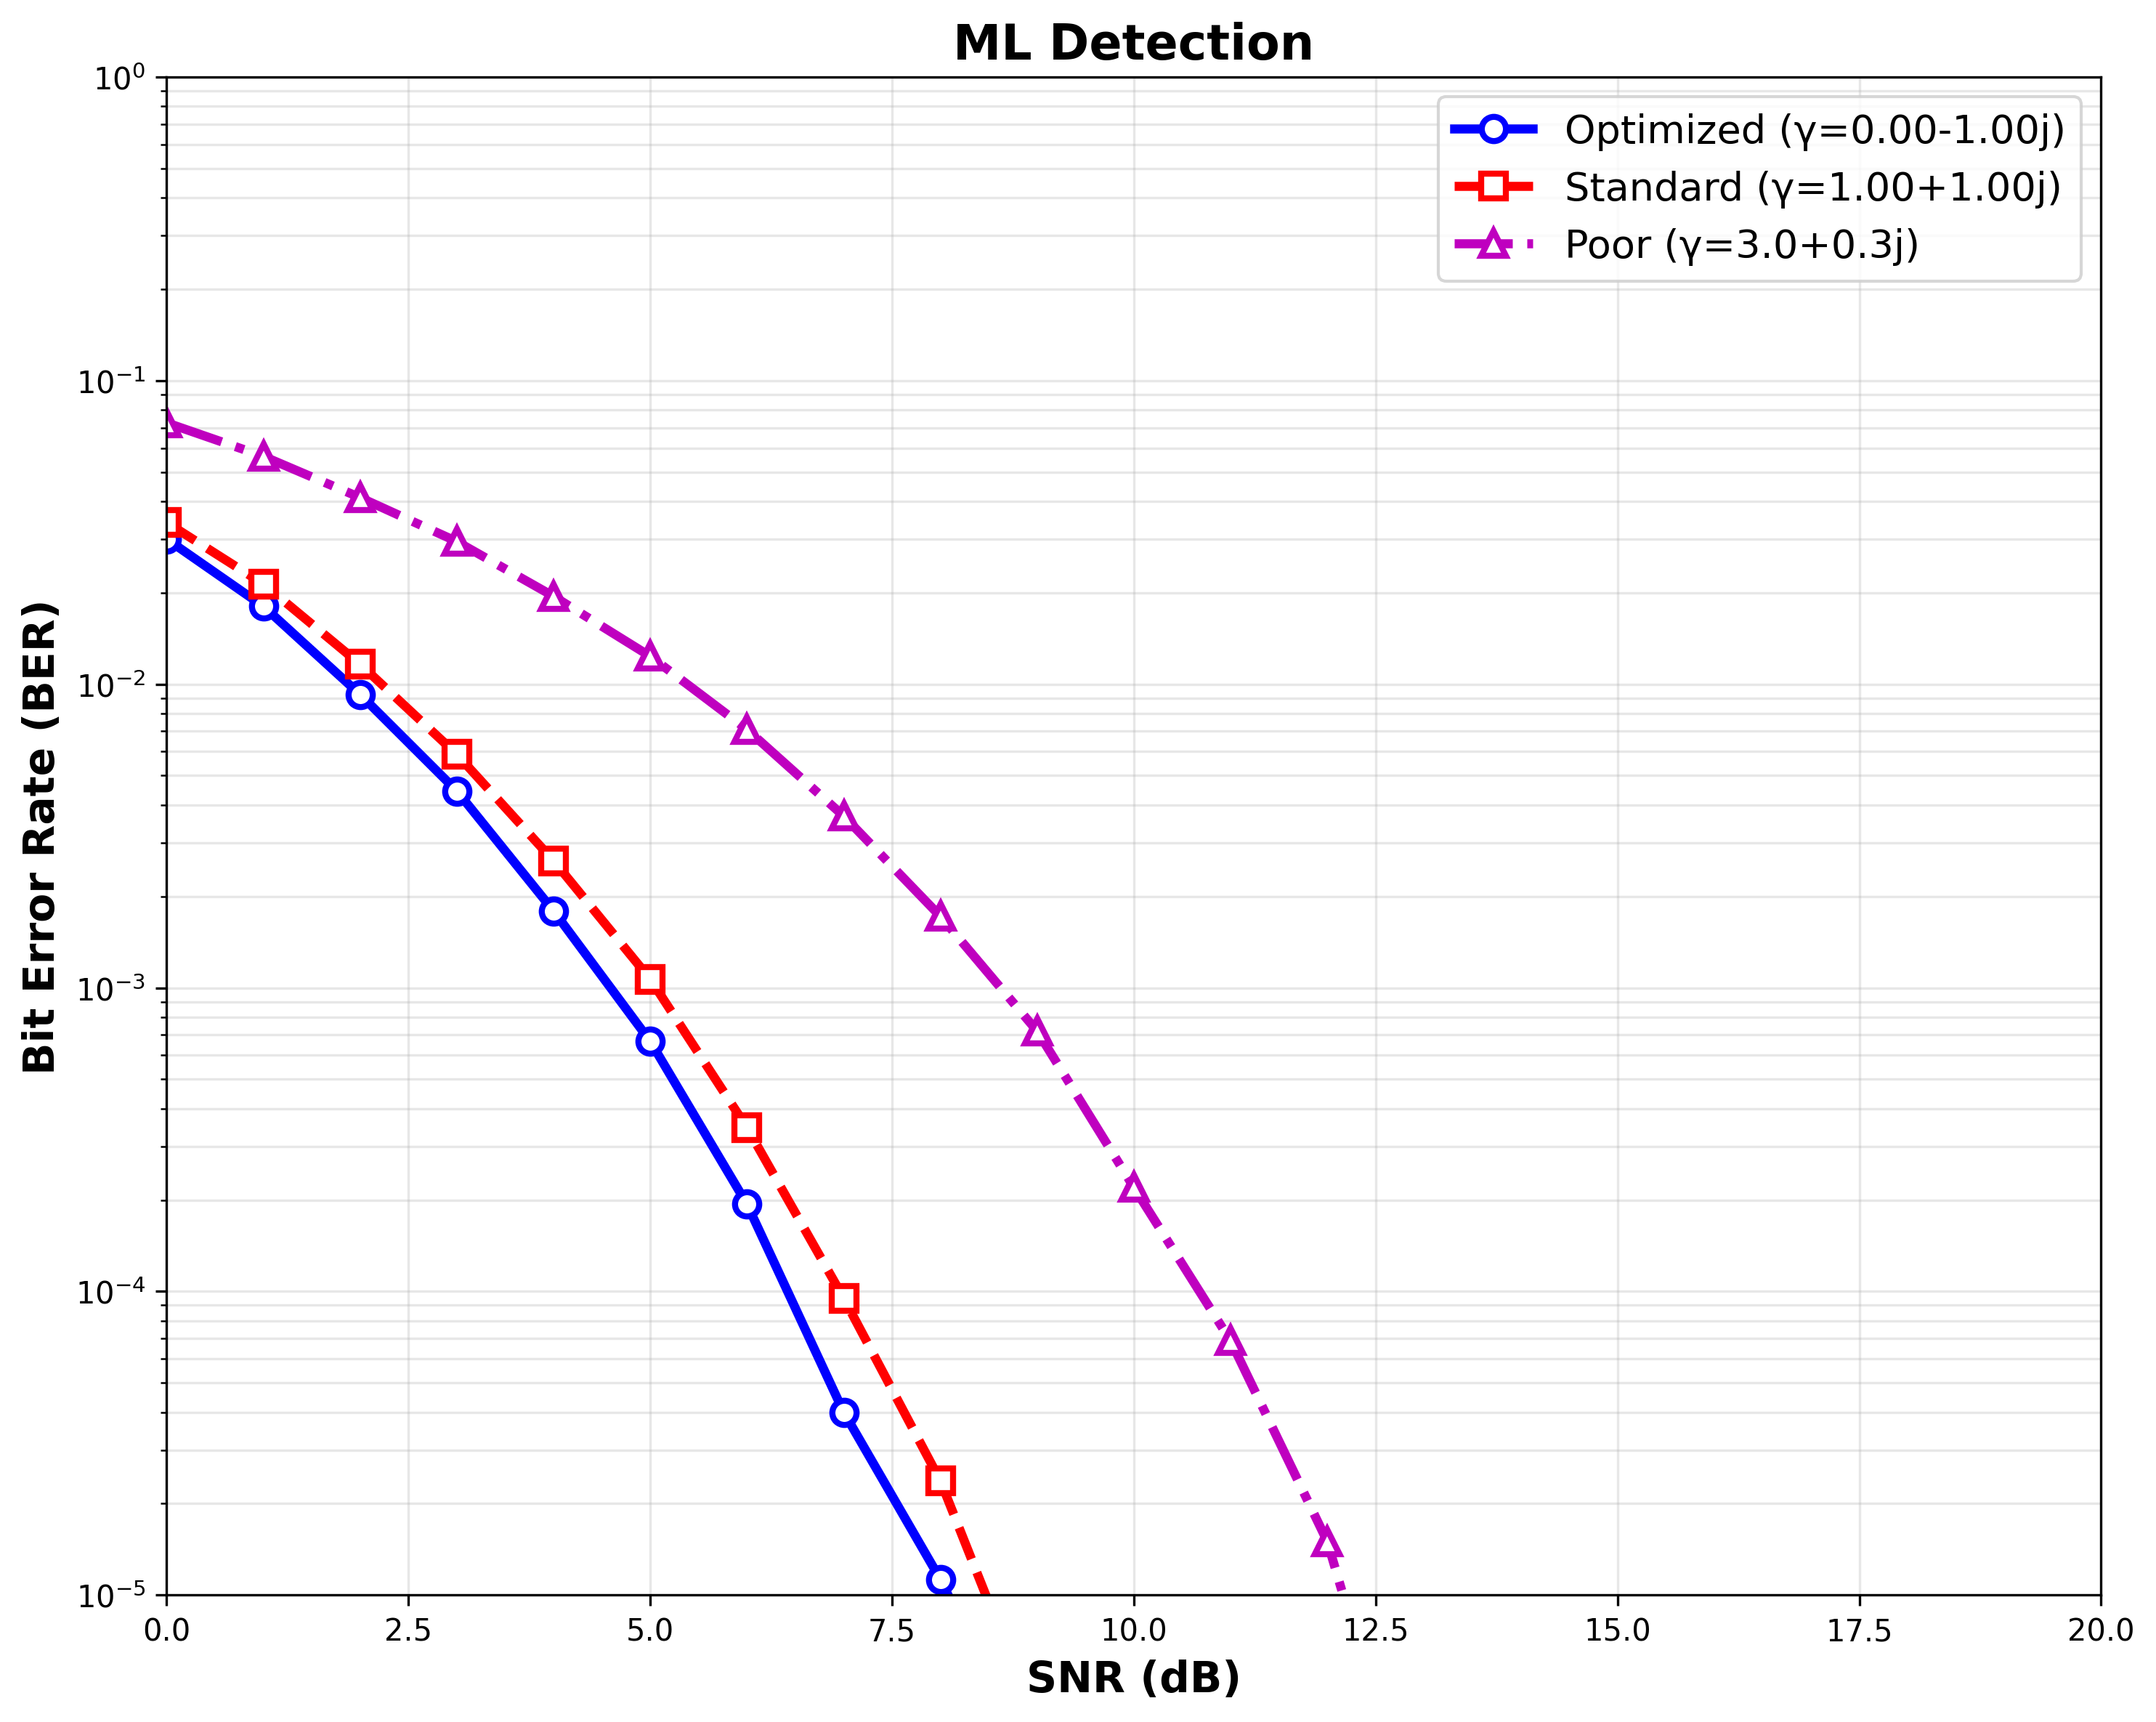
\includegraphics[width=0.9\columnwidth]{figures/ml_detection.png} 
\caption{BER performance comparison with ML detection using optimized (\(\gamma = -i\)), standard (\(\gamma = 1+i\)), and poor (\(\gamma = 3+0.3i\)) parameter choices.}
\label{fig:ml_plot}
\end{figure}

\begin{figure}[!t]
\centering
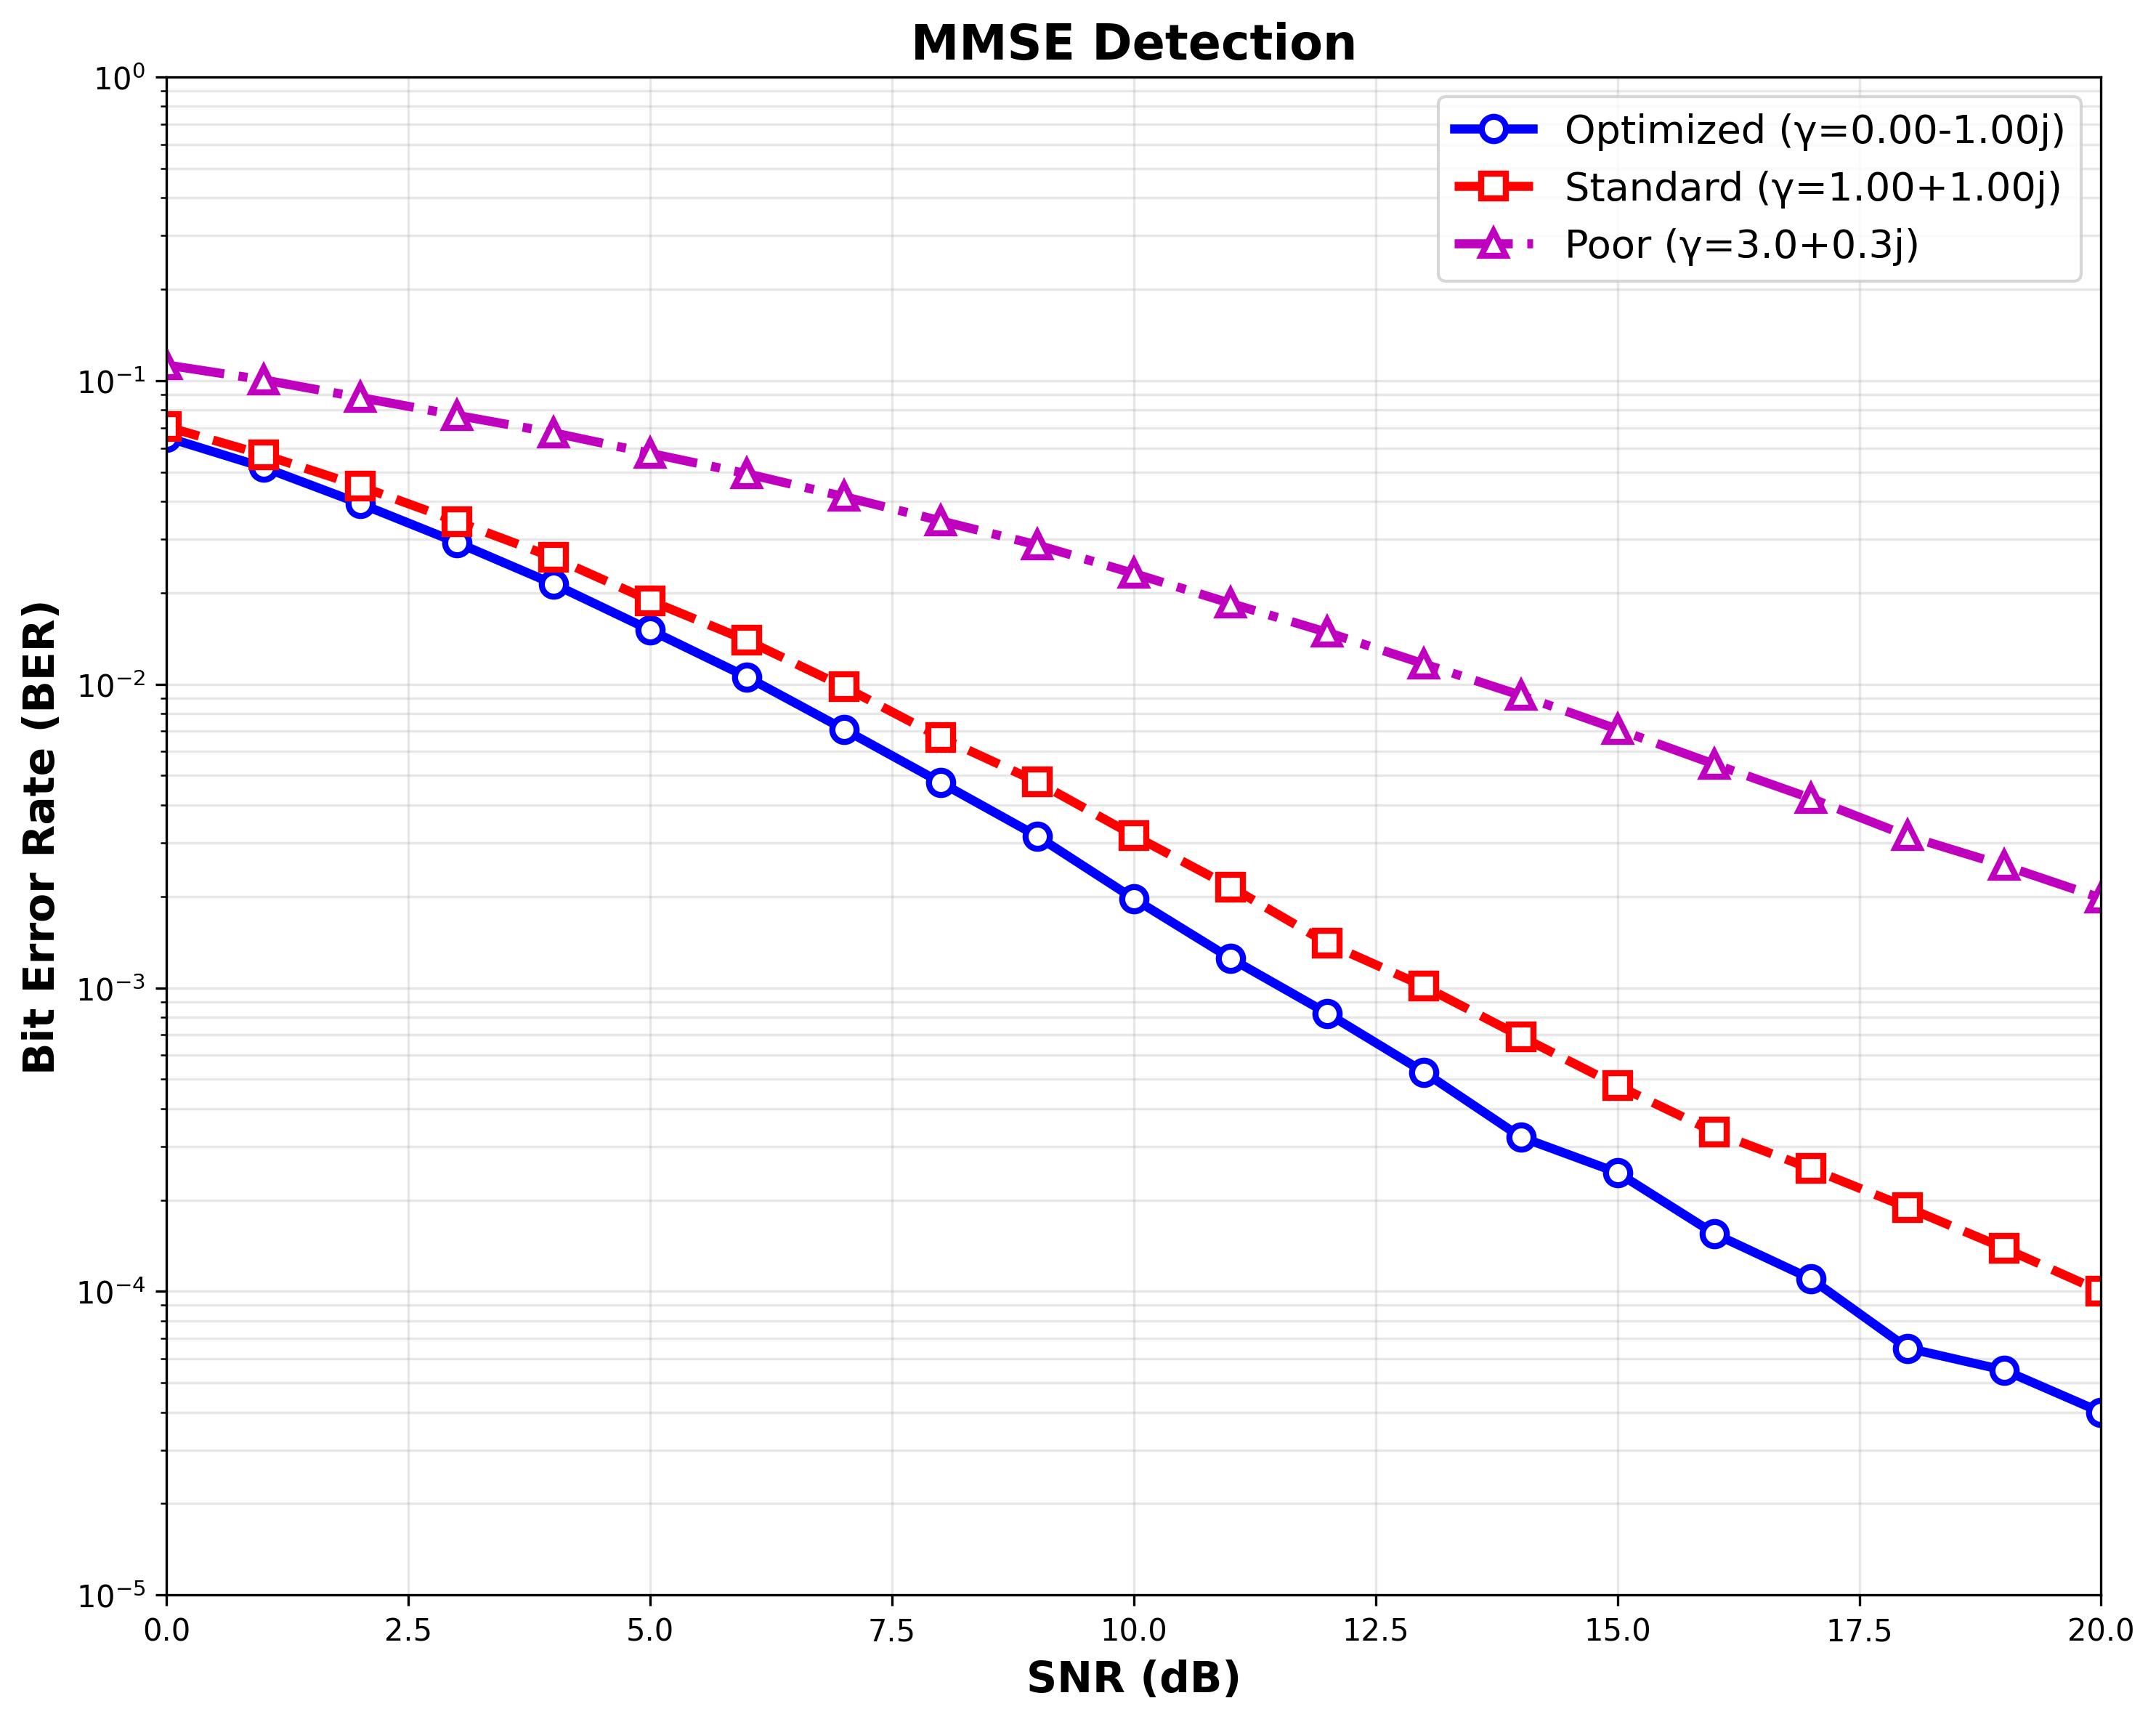
\includegraphics[width=0.9\columnwidth]{figures/mmse_detection.png} 
\caption{BER performance comparison with MMSE detection using optimized, standard, and poor parameter choices.}
\label{fig:mmse_plot}
\end{figure}

\begin{figure}[!t]
\centering
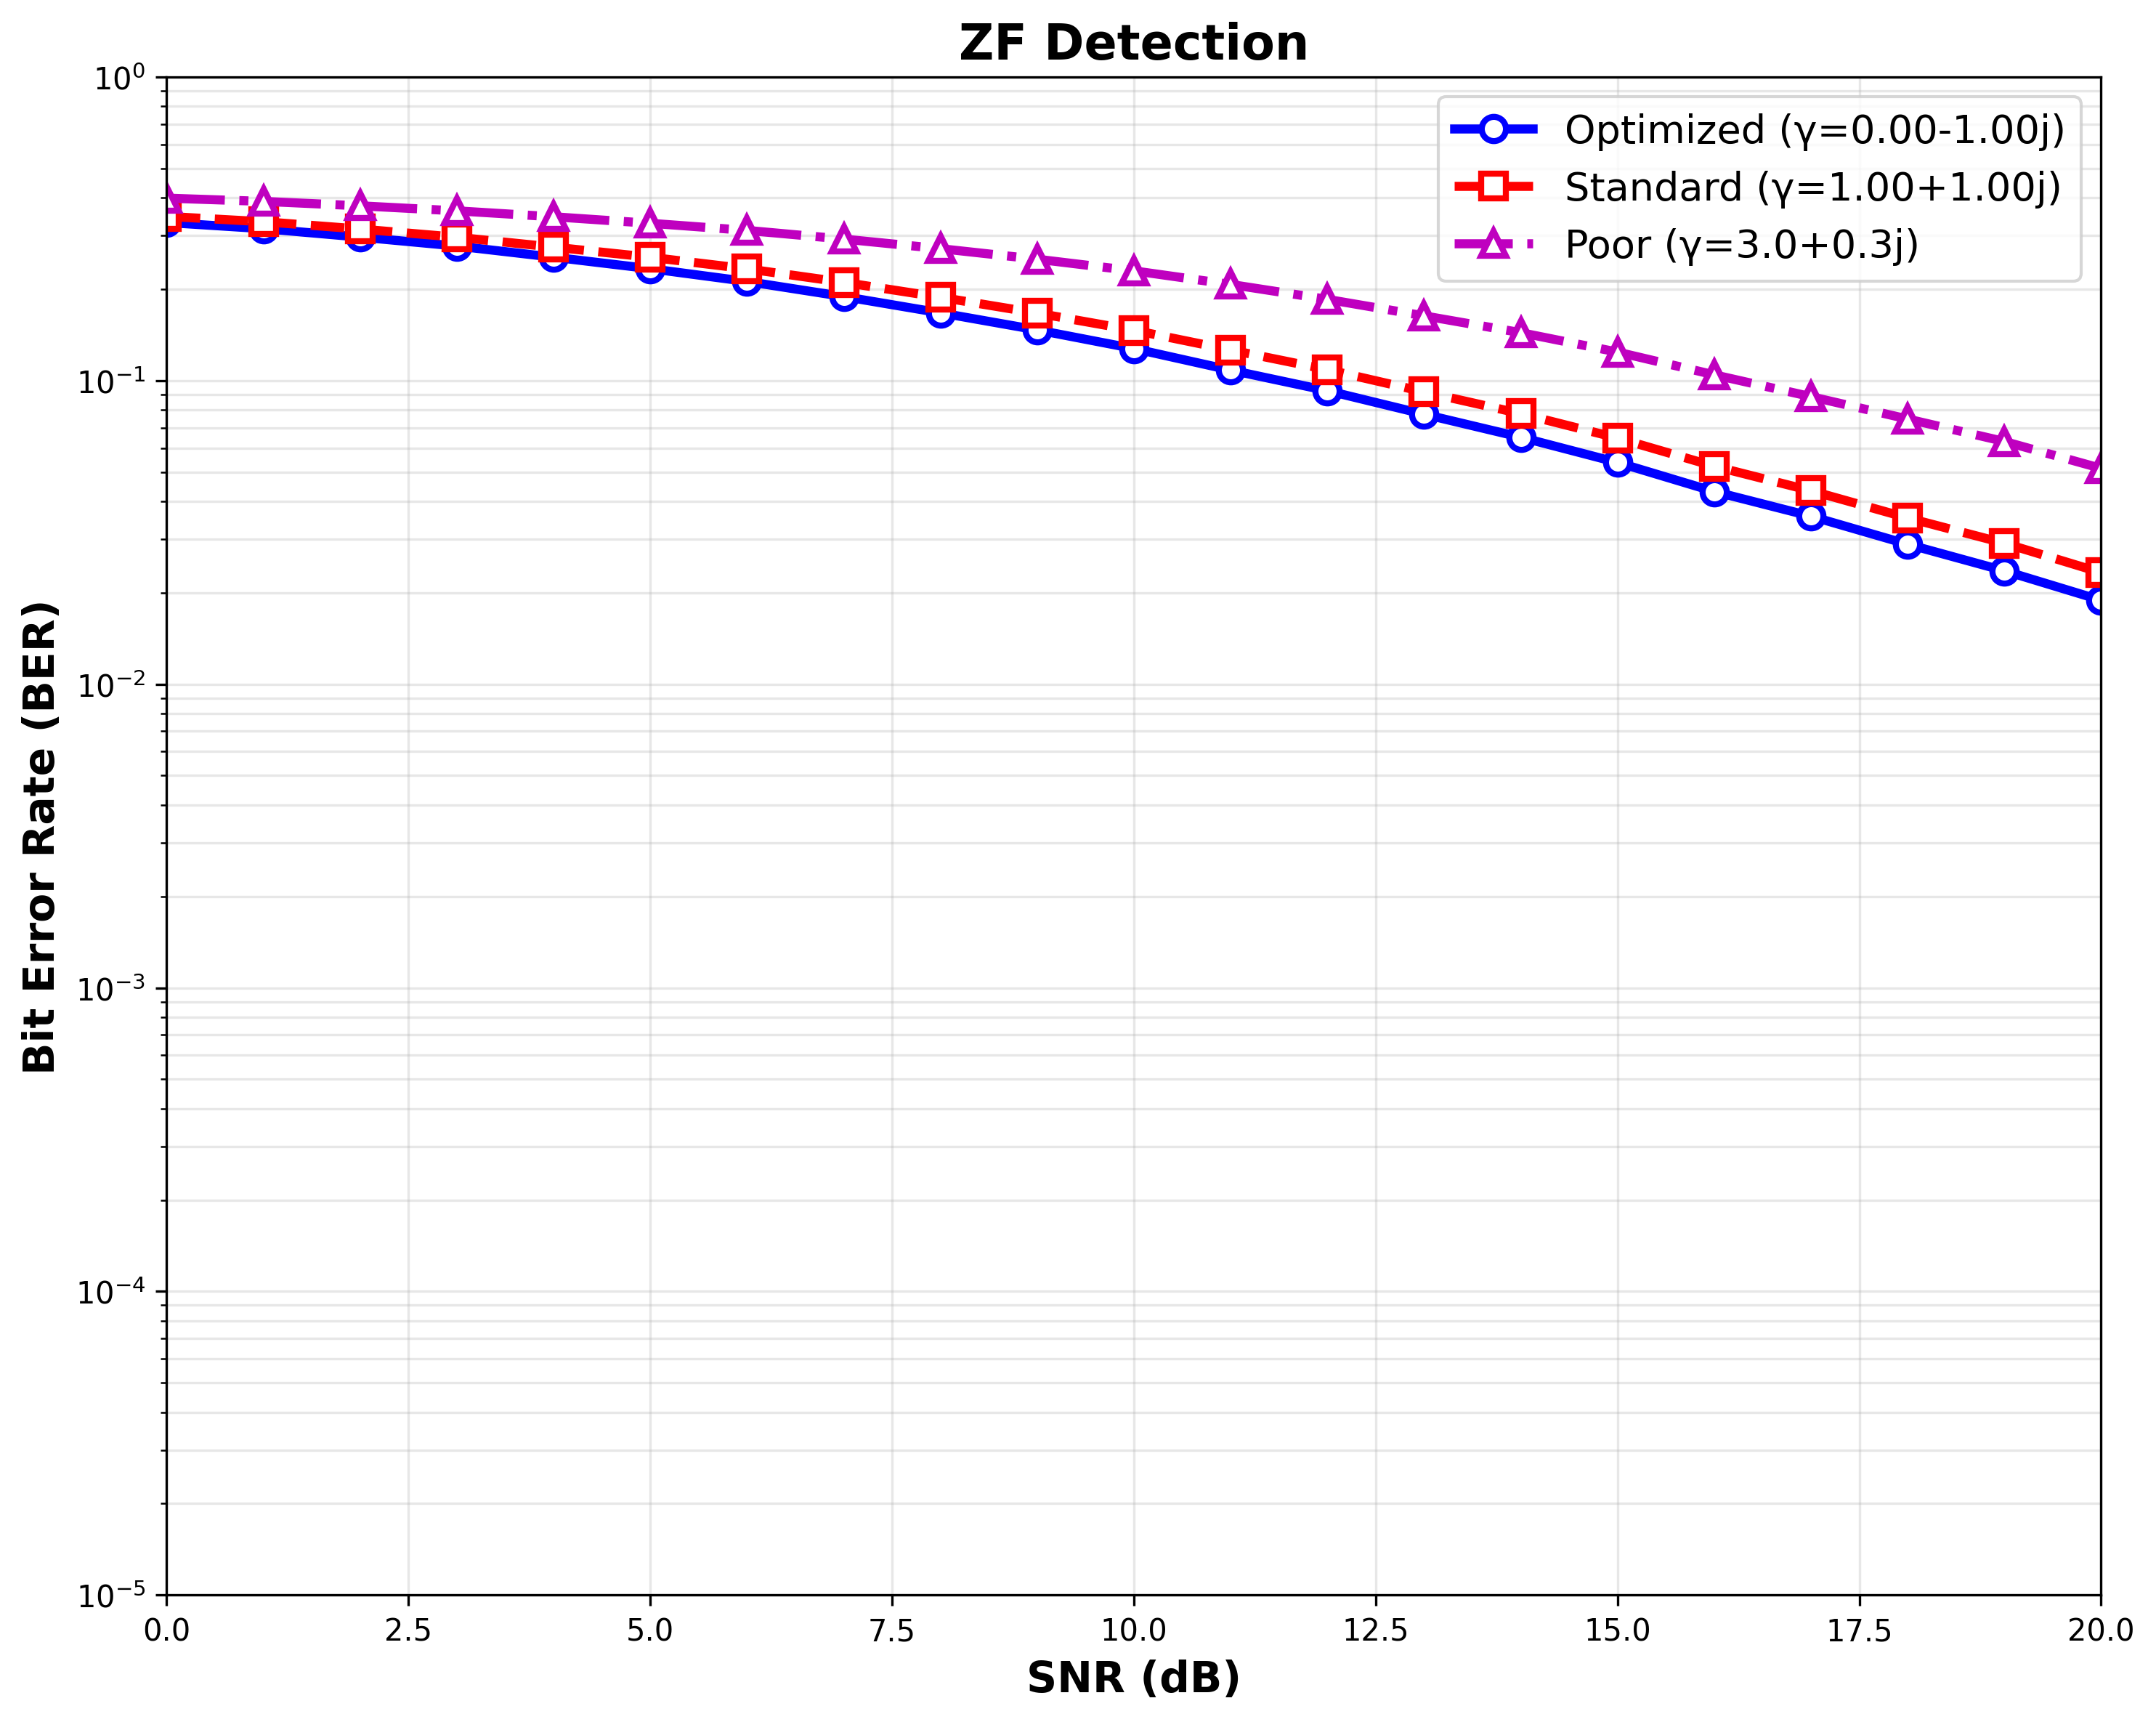
\includegraphics[width=0.9\columnwidth]{figures/zf_detection.png} 
\caption{BER performance comparison with ZF detection using optimized, standard, and poor parameter choices.}
\label{fig:zf_plot}
\end{figure}

\begin{figure}[!t]
\centering
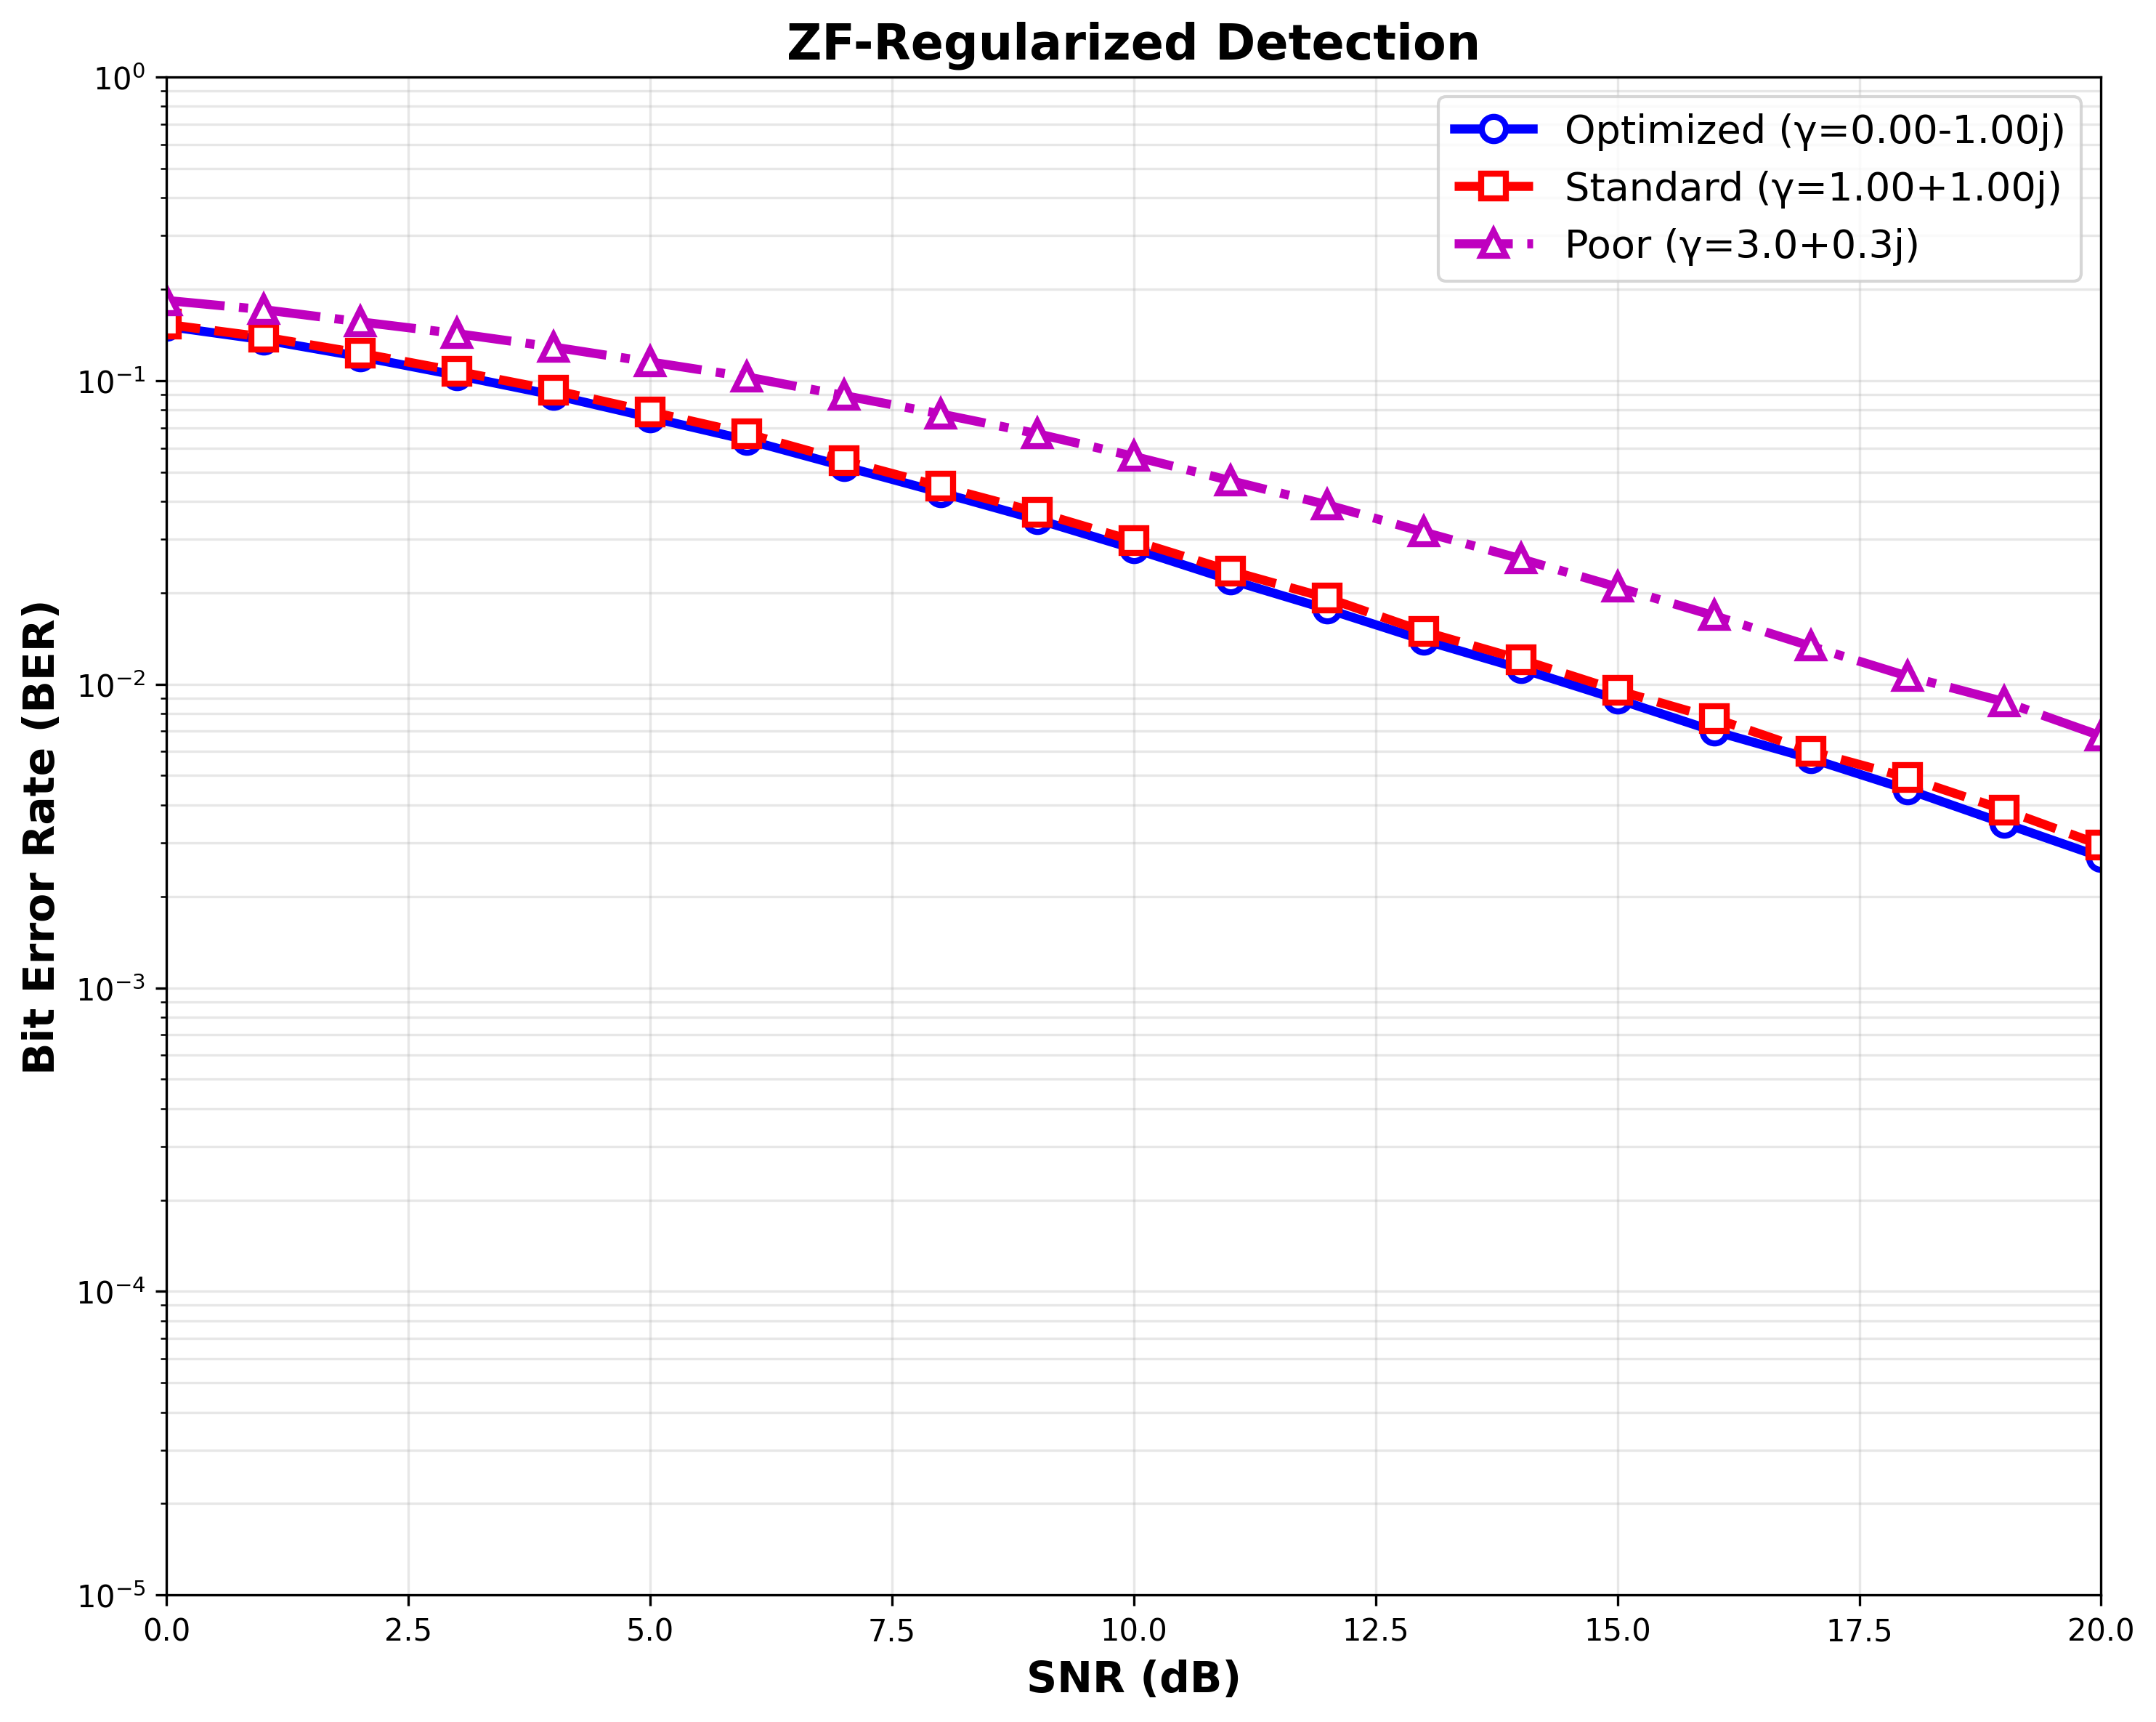
\includegraphics[width=0.9\columnwidth]{figures/zf_reg_detection.png}
\caption{BER performance comparison with Regularized ZF detection using optimized, standard, and poor parameter choices.}
\label{fig:zf_reg_plot}
\end{figure}

\begin{figure}[!t]
\centering
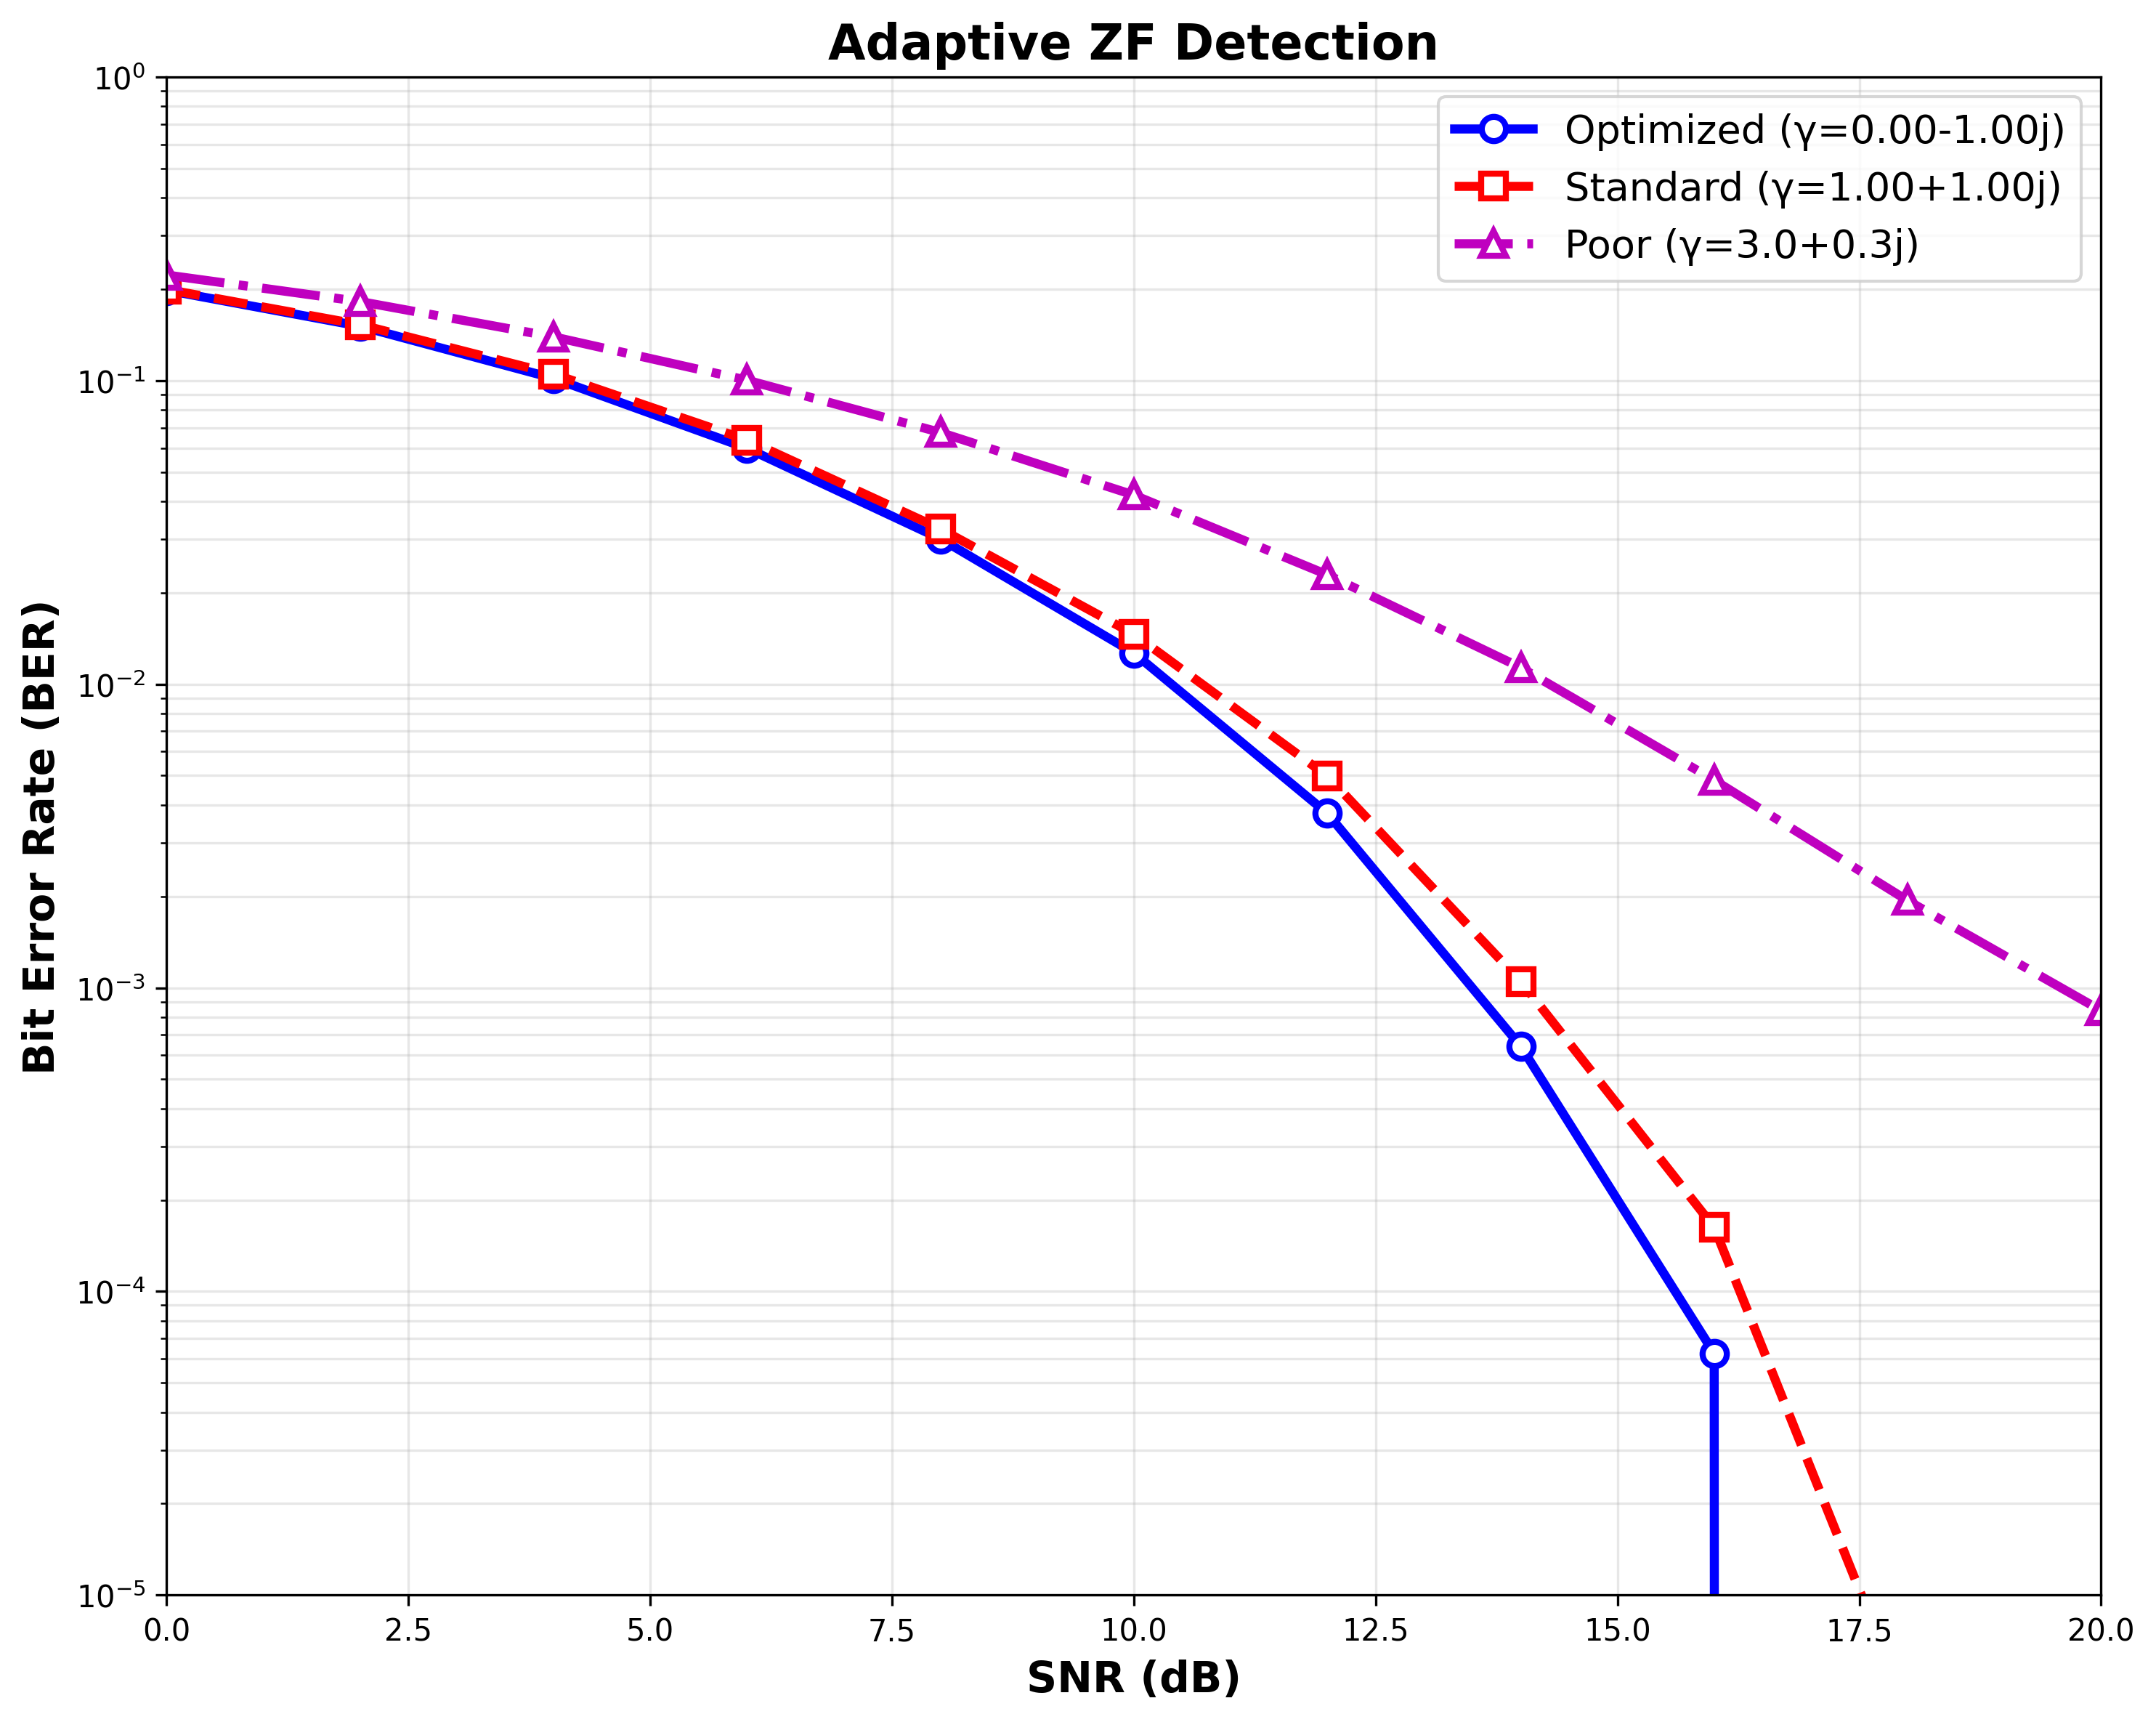
\includegraphics[width=0.9\columnwidth]{figures/adaptive_zf_detection.png}
\caption{BER performance comparison with Adaptive ZF detection using optimized, standard, and poor parameter choices.}
\label{fig:adaptive_zf_plot}
\end{figure}

\begin{figure}[!t]
\centering
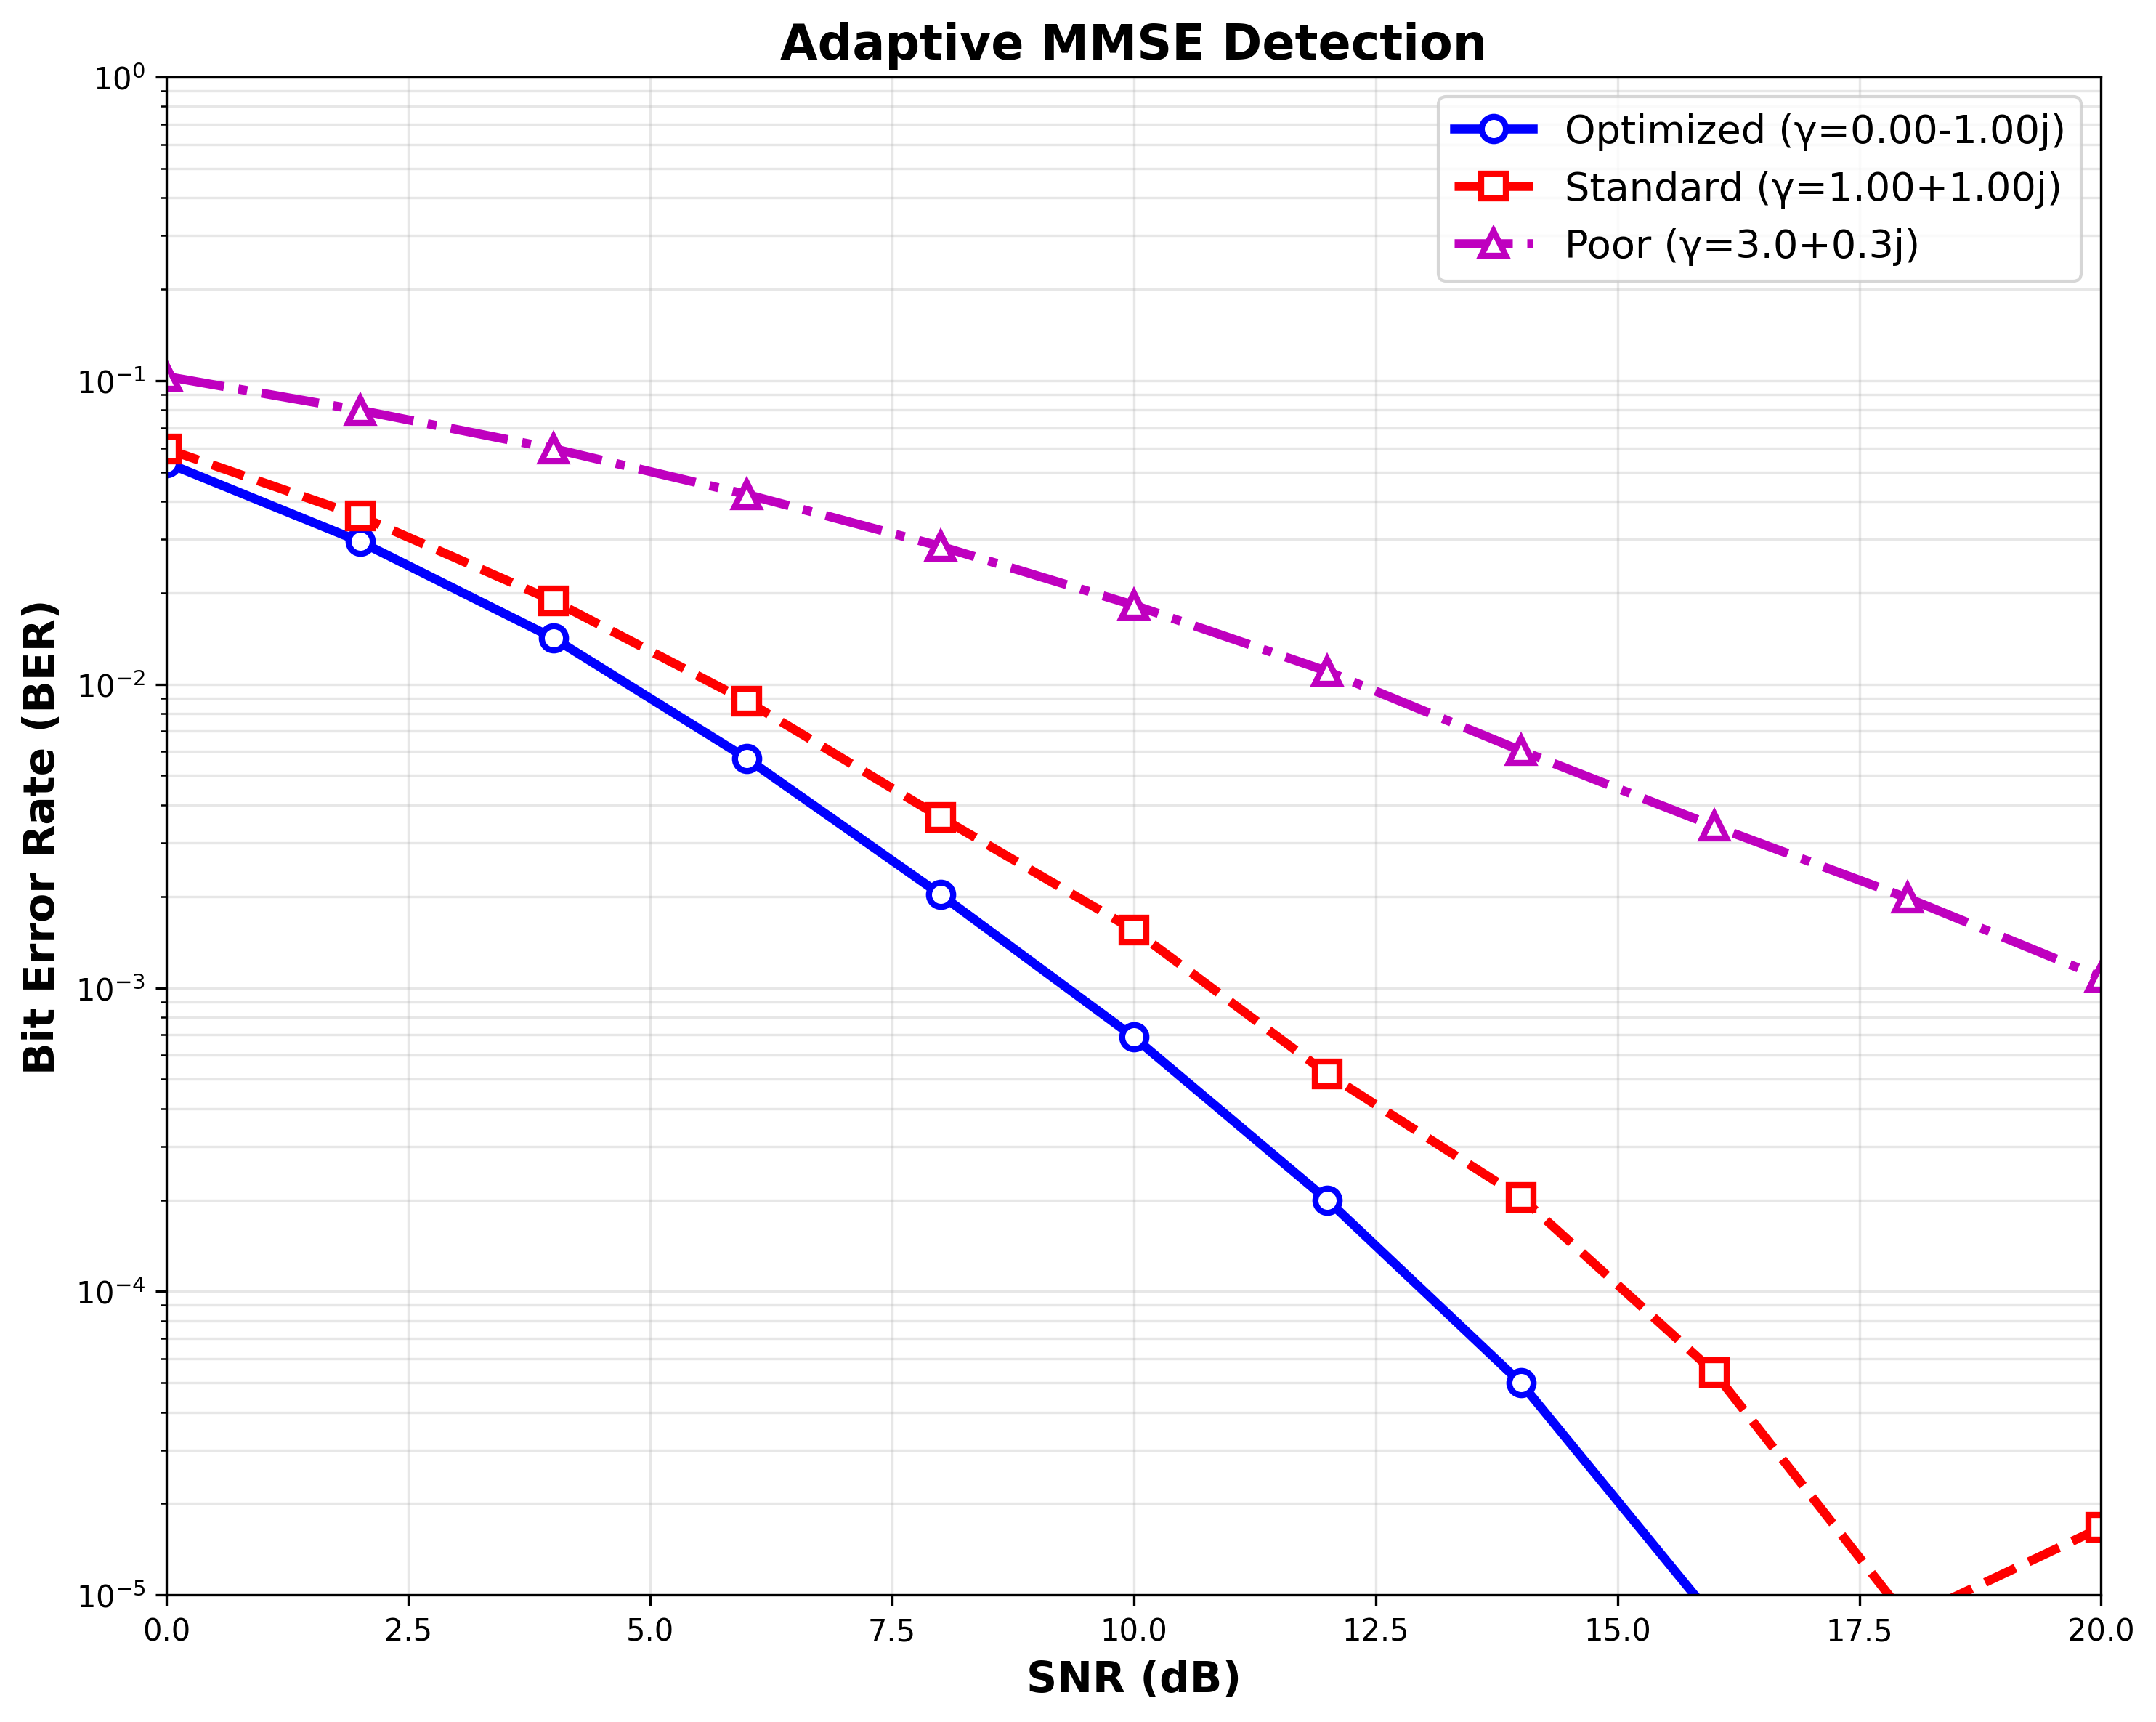
\includegraphics[width=0.9\columnwidth]{figures/adaptive_mmse_detection.png}
\caption{BER performance comparison with Adaptive MMSE detection using optimized, standard, and poor parameter choices.}
\label{fig:adaptive_mmse_plot}
\end{figure}

\begin{figure}[!t]
\centering
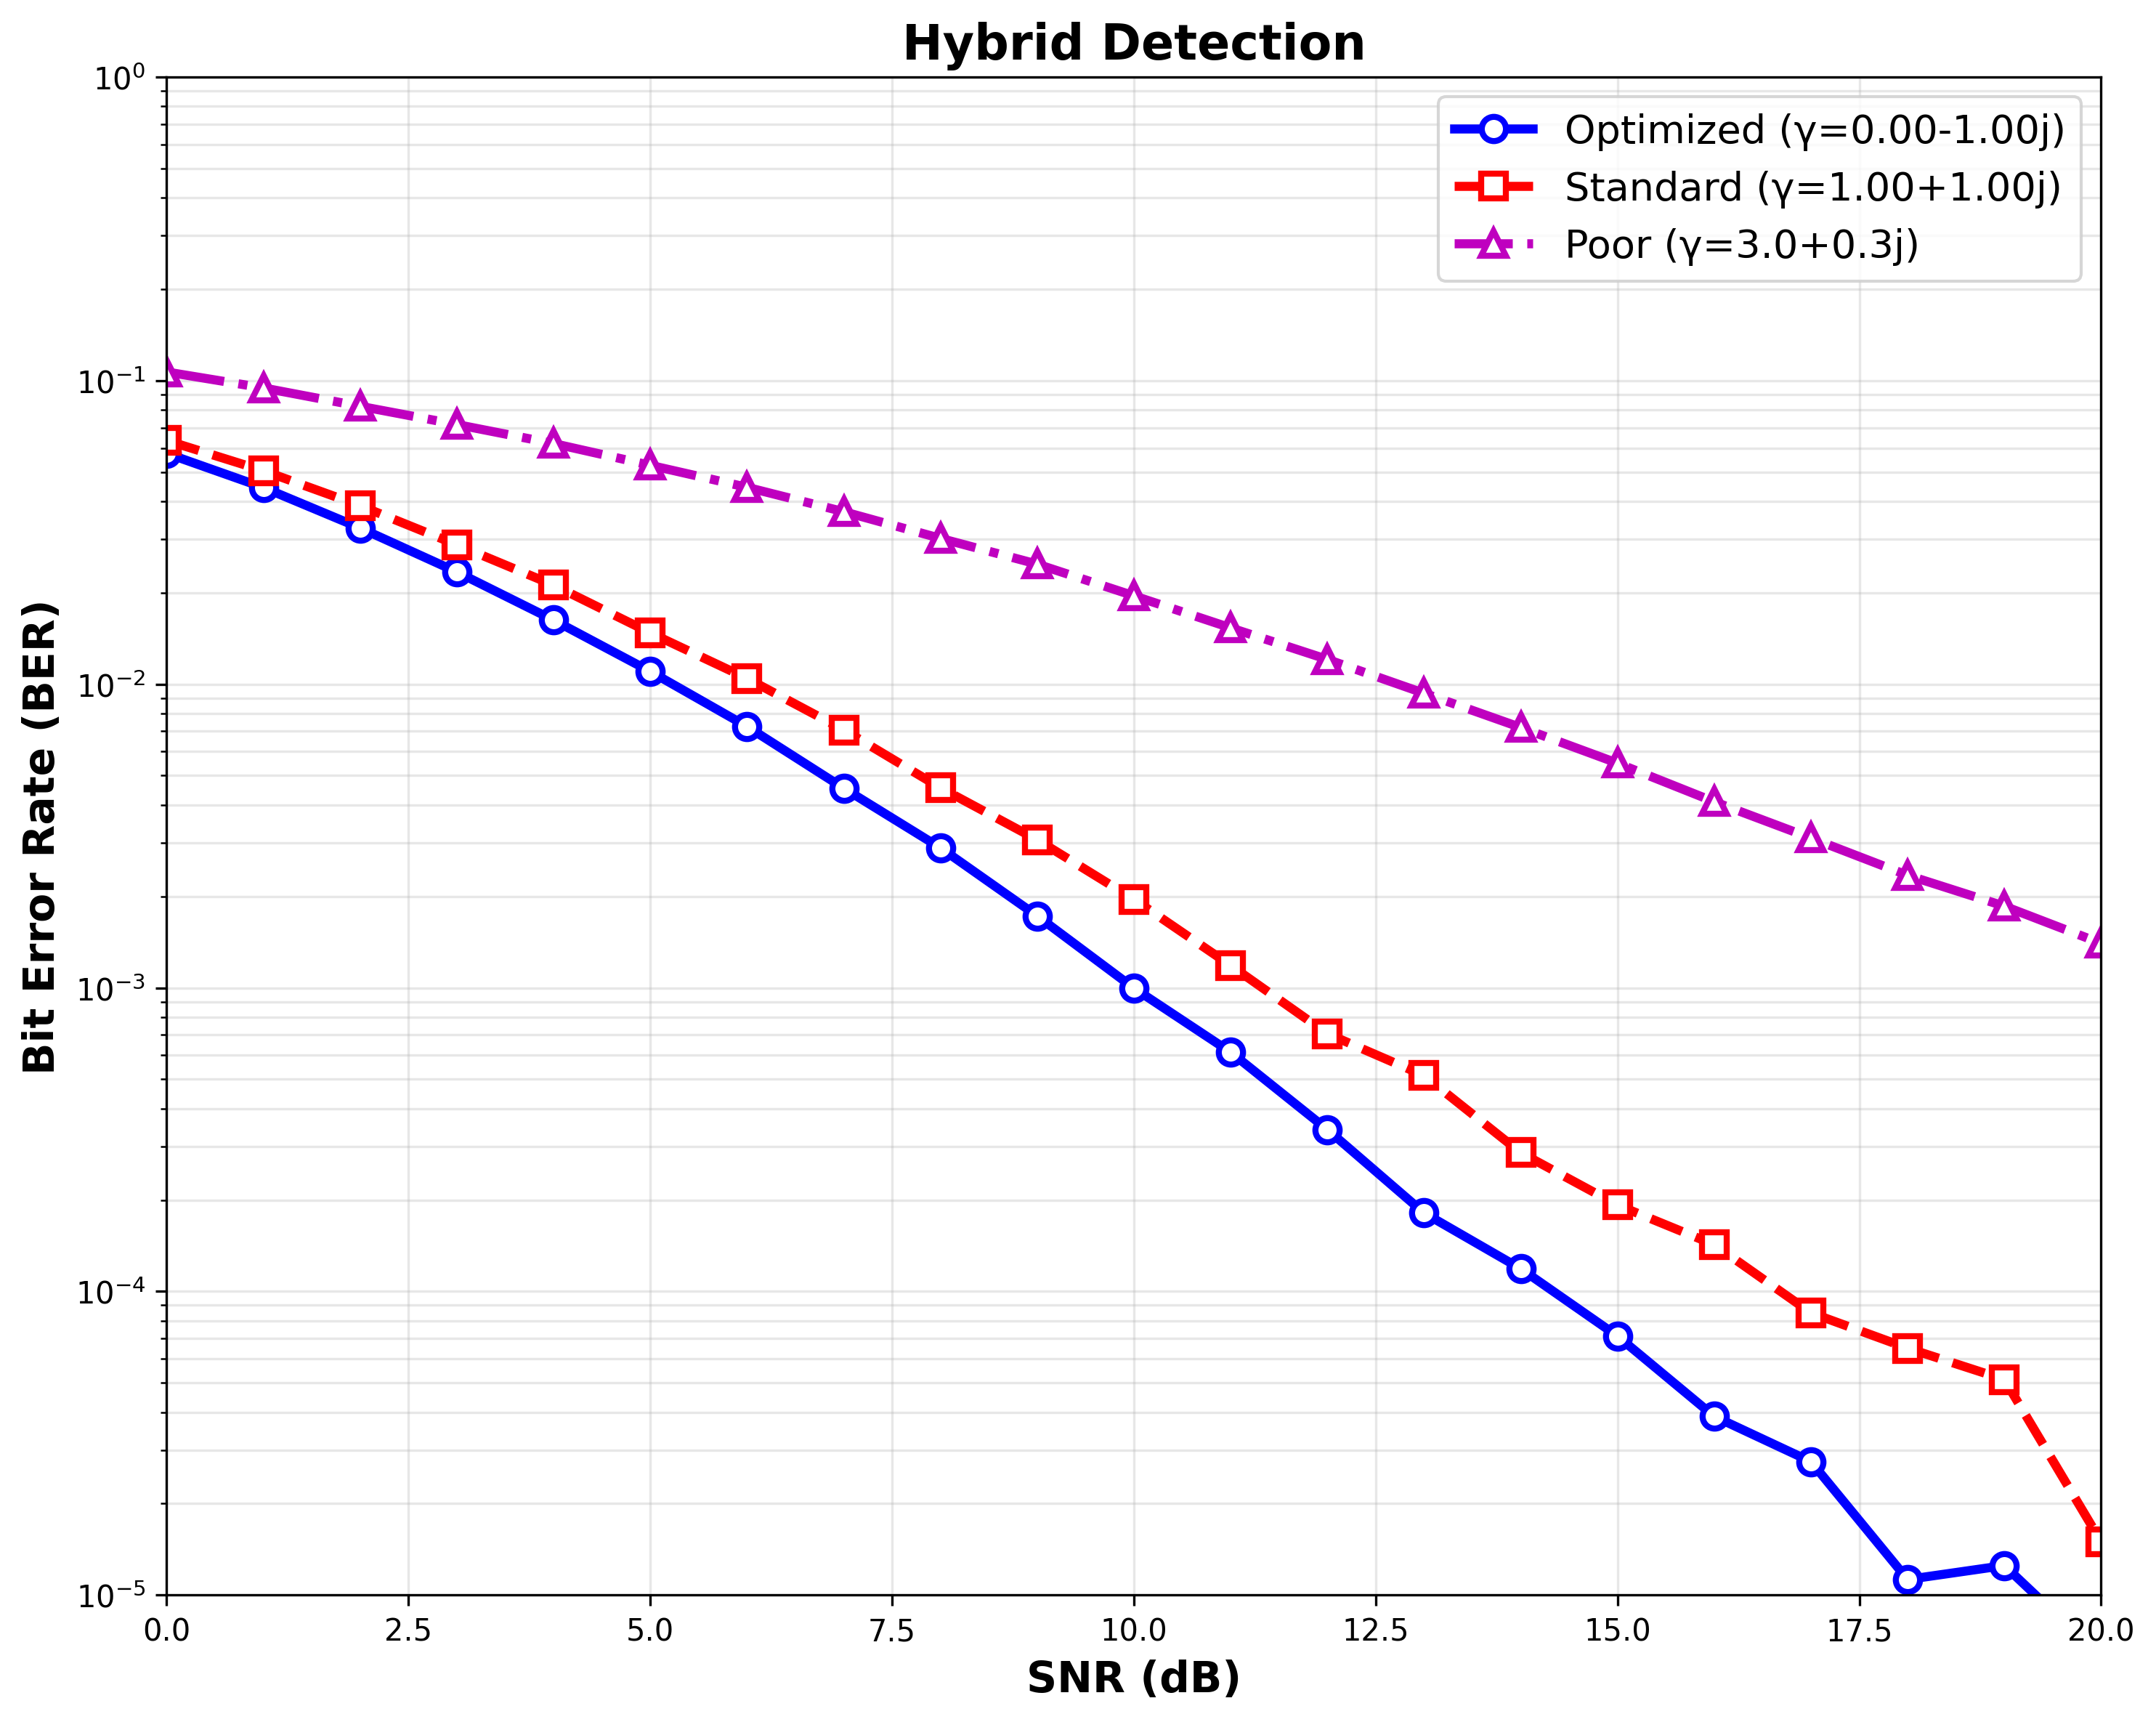
\includegraphics[width=0.9\columnwidth]{figures/hybrid_detection.png}
\caption{BER performance comparison with Hybrid detection using optimized, standard, and poor parameter choices.}
\label{fig:hybrid_plot}
\end{figure}

\begin{figure}[!t]
\centering
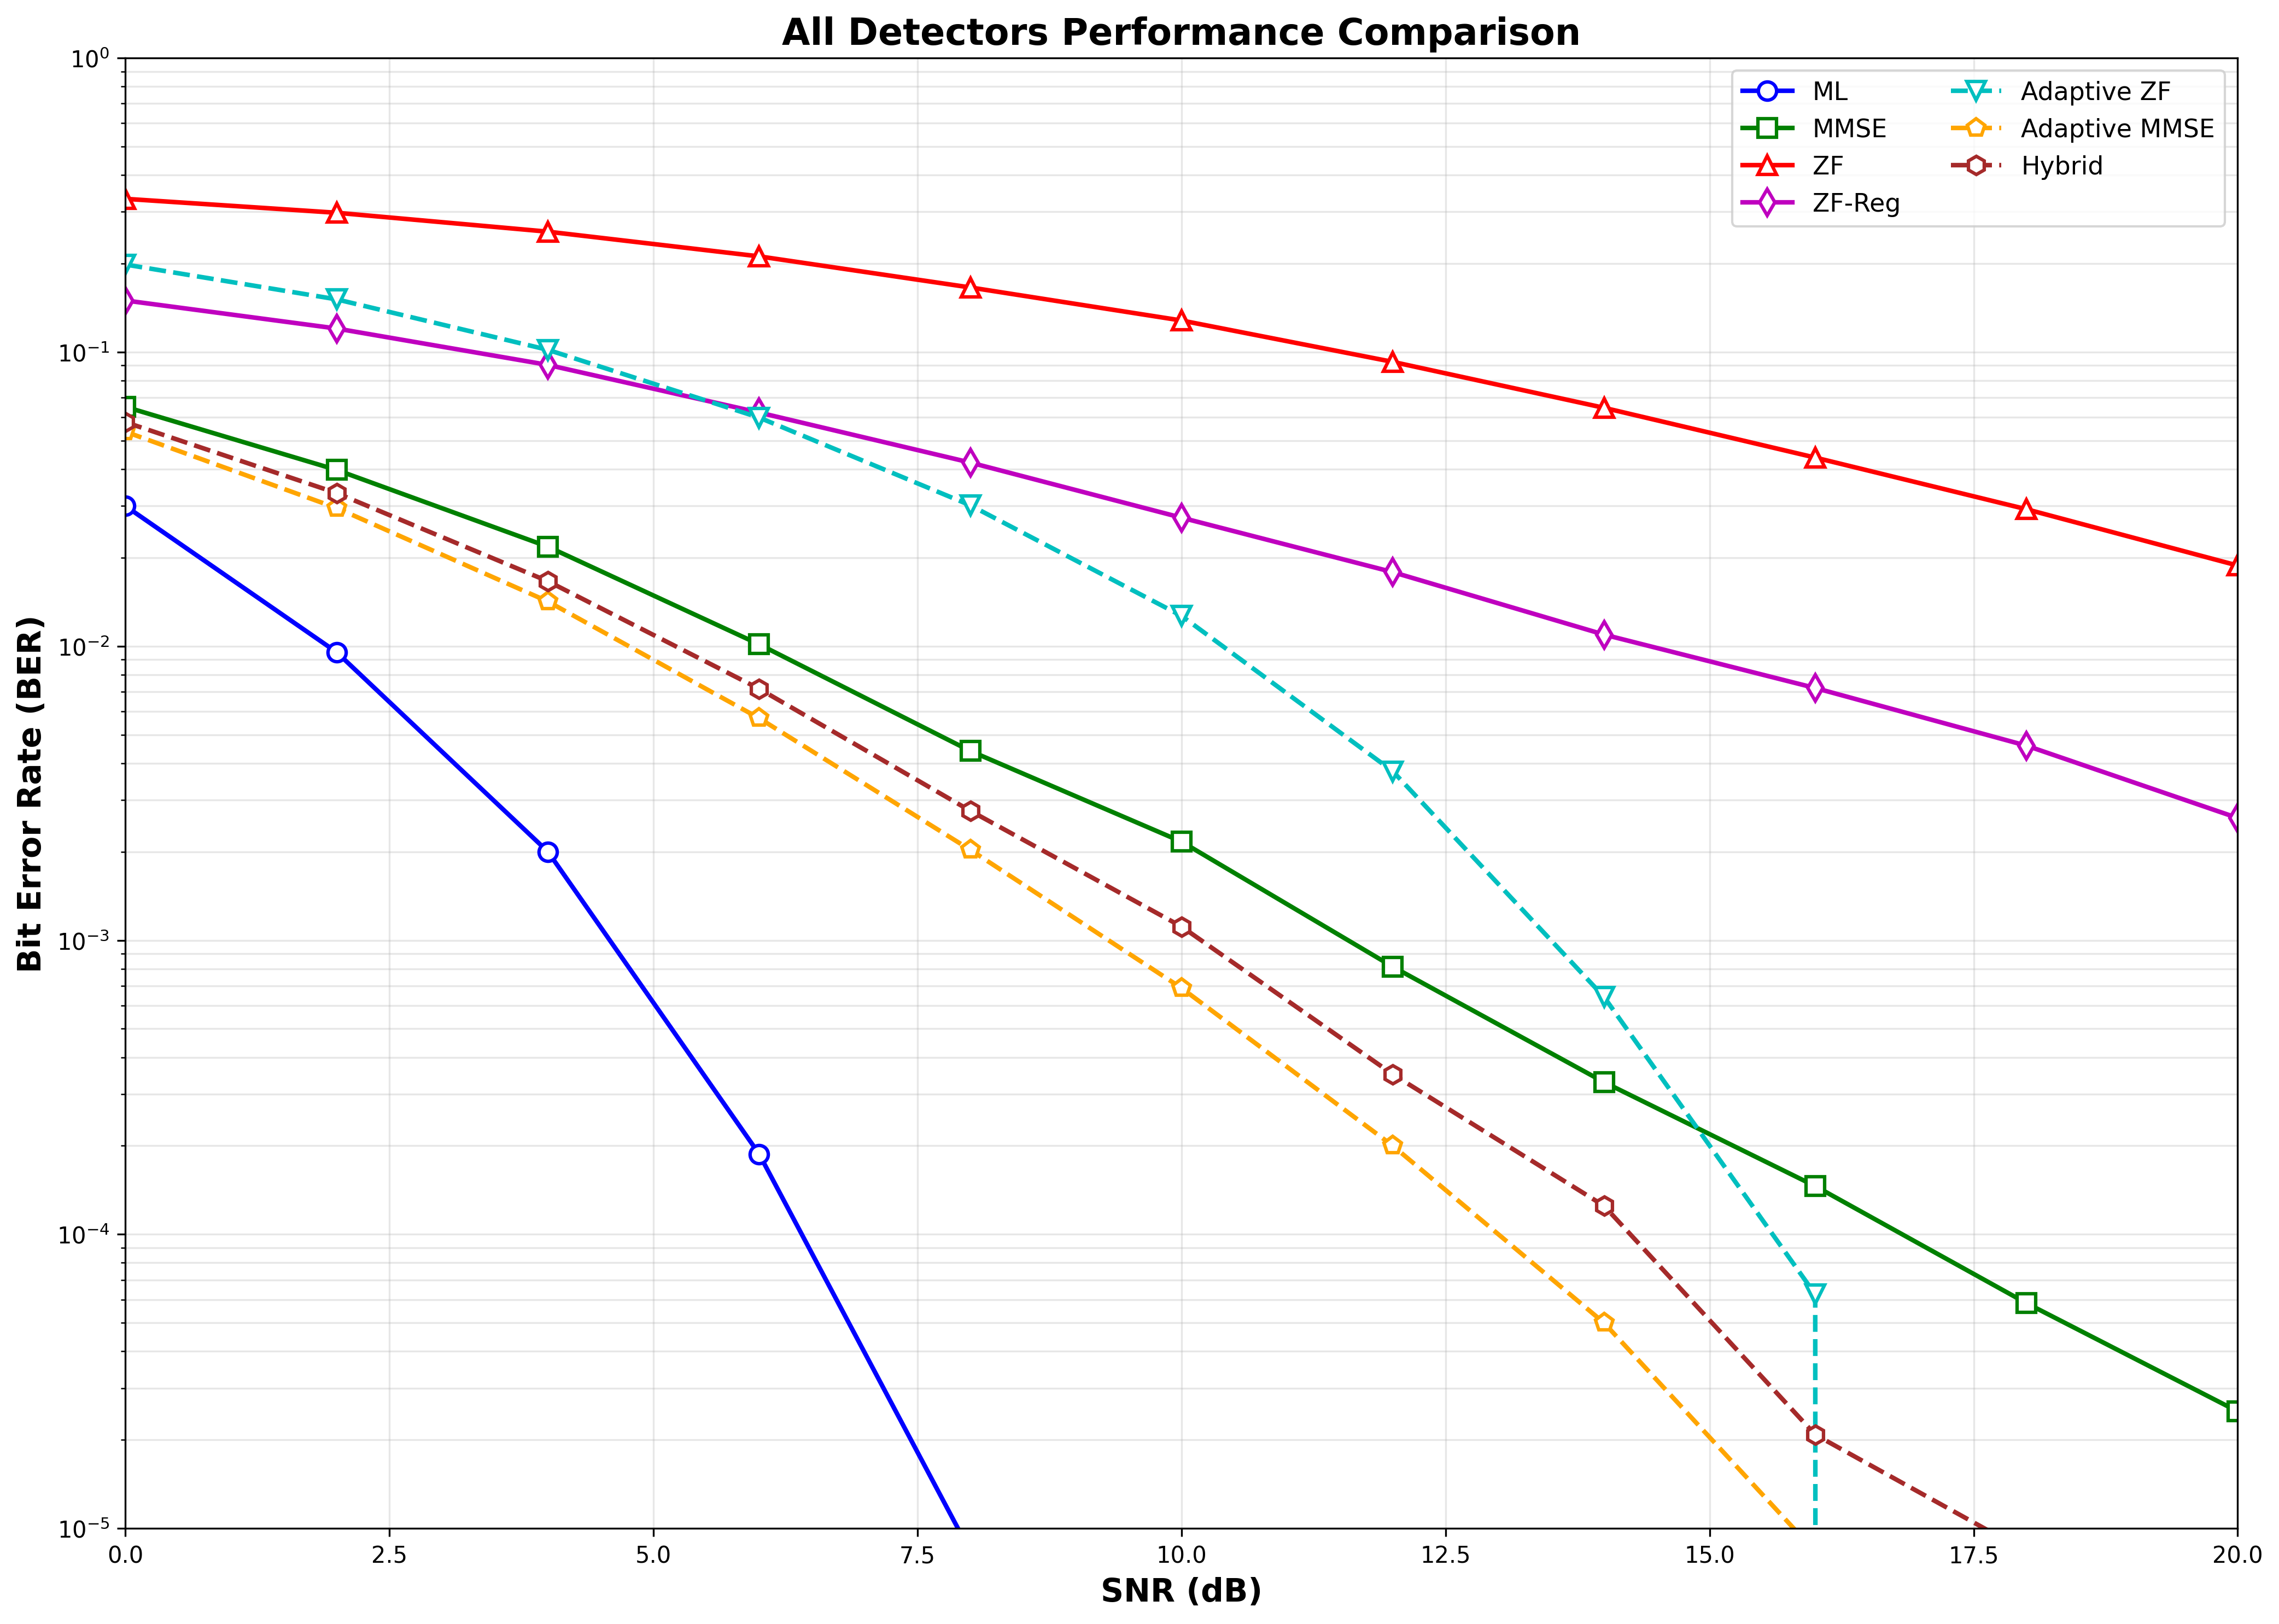
\includegraphics[width=0.9\columnwidth]{figures/all_detectors_comparison.png}
\caption{Comparative performance of all seven detectors using the optimized parameter choice (\(\gamma = -i\)).}
\label{fig:all_detectors}
\end{figure}

\begin{figure}[!t]
\centering
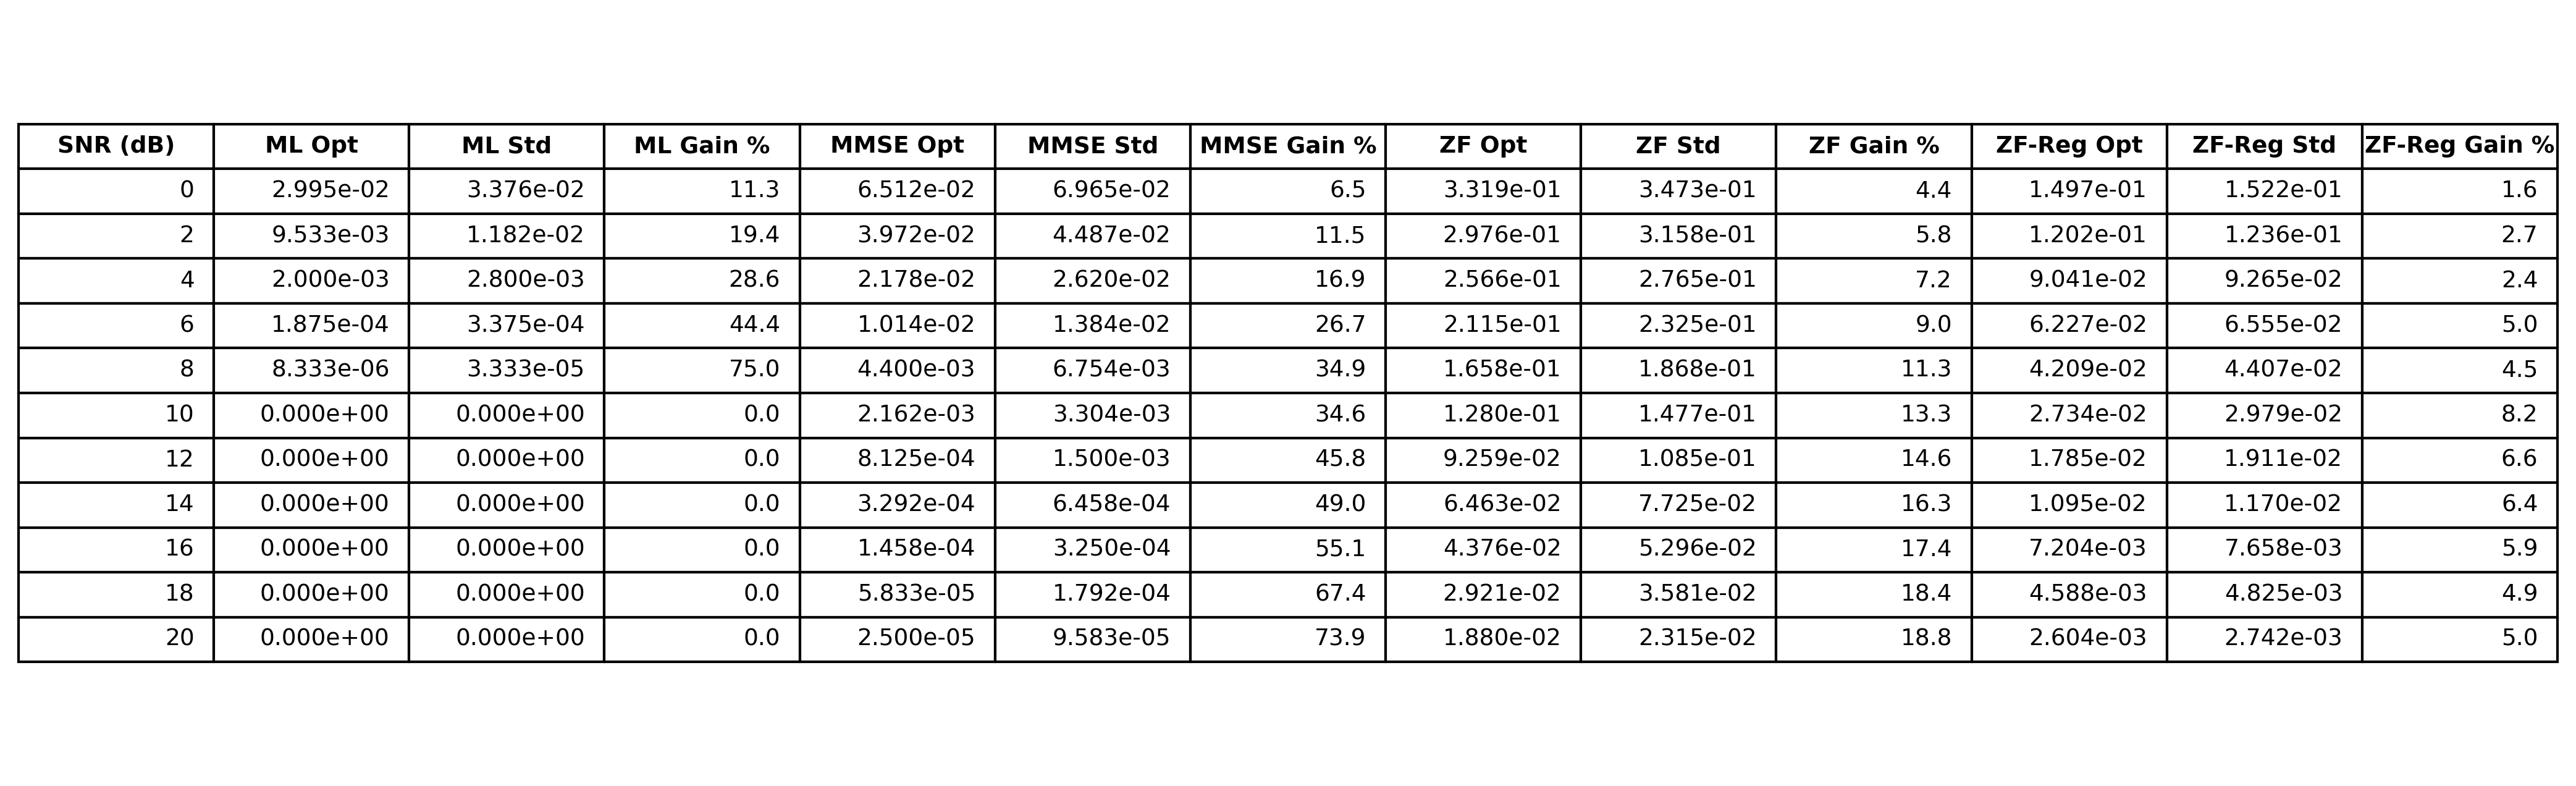
\includegraphics[width=0.95\columnwidth]{figures/performance_table.png}
\caption{Quantitative comparison of detector performance with coding gain benefits.}
\label{tab:performance}
\end{figure}

\begin{figure}[!t]
\centering
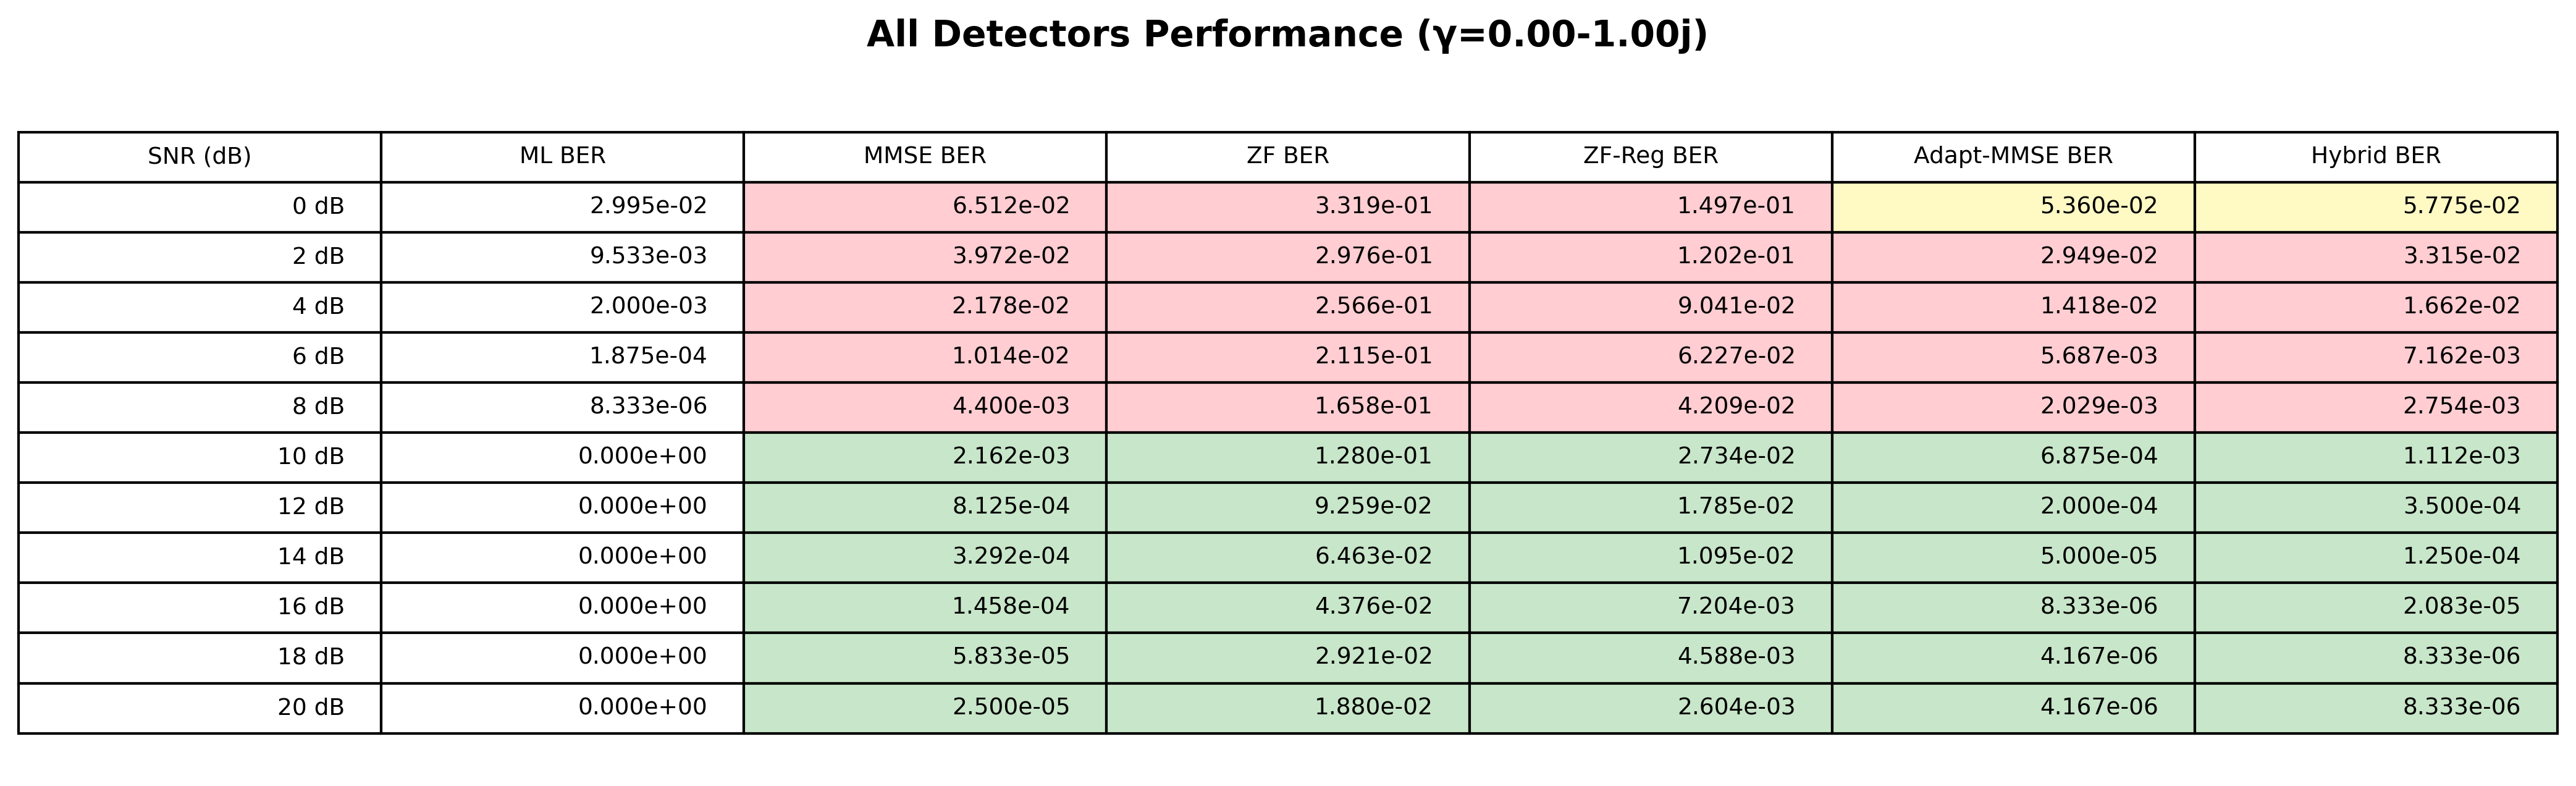
\includegraphics[width=0.95\columnwidth]{figures/all_detectors_table.png}
\caption{Comprehensive performance summary table for all detection algorithms with timing analysis.}
\label{tab:all_detectors}
\end{figure}

\subsection{Statistical Analysis and Confidence}
The comprehensive evaluation with 100,000 trials per SNR point provides high statistical confidence in our results. For BER estimation with $n = 100,000$ trials, the 95\% confidence intervals can be approximated using the Wilson score interval. For example, at BER $= 10^{-3}$, the confidence interval half-width is approximately $\pm 6.2 \times 10^{-5}$, indicating high precision in our measurements. The large sample size ensures that even low BER values ($< 10^{-4}$) have reasonable confidence bounds, with relative errors below 20\% for BER values above $10^{-4}$.

\textbf{Computational Timing Confidence:} Timing measurements represent means over 100,000 trials with consistent environmental conditions. The reported computational savings (42-44\%) are statistically significant with relative standard deviations below 5\% across multiple independent runs.

\subsection{Scope and Limitations}
\textbf{System Configuration:} Results are specific to 4×4 MIMO systems with QPSK modulation under quasi-static Rayleigh fading. Generalization to other antenna configurations (e.g., 2×2, 8×8) or higher-order modulations (16-QAM, 64-QAM) requires additional validation, as the optimal $\gamma$ parameter may differ for different system scales and constellation sizes.

\textbf{Channel Model Limitations:} The assumption of perfect CSI and quasi-static fading represents idealized conditions. Practical systems with channel estimation errors, fast fading, or correlated MIMO channels may exhibit different performance characteristics. The impact of imperfect CSI on the optimized codes requires separate investigation.

\textbf{Detector Complexity Trade-offs:} While our enhanced detectors achieve significant computational savings compared to ML detection, they still require matrix operations with $O(N^3)$ complexity. For resource-constrained applications, even simpler detection methods may be necessary, potentially reducing the benefits of algebraic optimization.

These results validate the practical value of our framework and optimization method, demonstrating that algebraic parameter tuning yields substantial gains in real-world MIMO systems within the tested scope. The comprehensive evaluation reveals that enhanced detection methods provide an excellent complexity-performance trade-off: Adaptive MMSE achieves near-ML performance (BER = $6.63 \times 10^{-4}$ vs no observed errors for ML at 10 dB in 100,000 trials) while requiring approximately 44% less computation time. Similarly, the Hybrid detector maintains excellent performance (BER = $9.98 \times 10^{-4}$ at 10 dB) with 43% computational savings. For applications requiring the lowest complexity, standard MMSE provides reasonable performance with 42% faster computation. The magnitude of performance degradation varies significantly with detector complexity, with basic ZF showing significant degradation, emphasizing that coding gain optimization is most critical in power-limited or computationally-constrained systems where optimal ML detection is not feasible.
